\documentclass[11pt]{article}

    \usepackage[breakable]{tcolorbox}
    \usepackage{parskip} % Stop auto-indenting (to mimic markdown behaviour)
    
    \usepackage{iftex}
    \ifPDFTeX
    	\usepackage[T1]{fontenc}
    	\usepackage{mathpazo}
    \else
    	\usepackage{fontspec}
    \fi

    % Basic figure setup, for now with no caption control since it's done
    % automatically by Pandoc (which extracts ![](path) syntax from Markdown).
    \usepackage{graphicx}
    % Maintain compatibility with old templates. Remove in nbconvert 6.0
    \let\Oldincludegraphics\includegraphics
    % Ensure that by default, figures have no caption (until we provide a
    % proper Figure object with a Caption API and a way to capture that
    % in the conversion process - todo).
    \usepackage{caption}
    \DeclareCaptionFormat{nocaption}{}
    \captionsetup{format=nocaption,aboveskip=0pt,belowskip=0pt}

    \usepackage[Export]{adjustbox} % Used to constrain images to a maximum size
    \adjustboxset{max size={0.9\linewidth}{0.9\paperheight}}
    \usepackage{float}
    \floatplacement{figure}{H} % forces figures to be placed at the correct location
    \usepackage{xcolor} % Allow colors to be defined
    \usepackage{enumerate} % Needed for markdown enumerations to work
    \usepackage{geometry} % Used to adjust the document margins
    \usepackage{amsmath} % Equations
    \usepackage{amssymb} % Equations
    \usepackage{textcomp} % defines textquotesingle
    % Hack from http://tex.stackexchange.com/a/47451/13684:
    \AtBeginDocument{%
        \def\PYZsq{\textquotesingle}% Upright quotes in Pygmentized code
    }
    \usepackage{upquote} % Upright quotes for verbatim code
    \usepackage{eurosym} % defines \euro
    \usepackage[mathletters]{ucs} % Extended unicode (utf-8) support
    \usepackage{fancyvrb} % verbatim replacement that allows latex

    % The hyperref package gives us a pdf with properly built
    % internal navigation ('pdf bookmarks' for the table of contents,
    % internal cross-reference links, web links for URLs, etc.)
    \usepackage{hyperref}
    % The default LaTeX title has an obnoxious amount of whitespace. By default,
    % titling removes some of it. It also provides customization options.
    \usepackage{titling}
    \usepackage{longtable} % longtable support required by pandoc >1.10
    \usepackage{booktabs}  % table support for pandoc > 1.12.2
    \usepackage[inline]{enumitem} % IRkernel/repr support (it uses the enumerate* environment)
    \usepackage[normalem]{ulem} % ulem is needed to support strikethroughs (\sout)
                                % normalem makes italics be italics, not underlines
    \usepackage{mathrsfs}
    

    
    % Colors for the hyperref package
    \definecolor{urlcolor}{rgb}{0,.145,.698}
    \definecolor{linkcolor}{rgb}{.71,0.21,0.01}
    \definecolor{citecolor}{rgb}{.12,.54,.11}

    % ANSI colors
    \definecolor{ansi-black}{HTML}{3E424D}
    \definecolor{ansi-black-intense}{HTML}{282C36}
    \definecolor{ansi-red}{HTML}{E75C58}
    \definecolor{ansi-red-intense}{HTML}{B22B31}
    \definecolor{ansi-green}{HTML}{00A250}
    \definecolor{ansi-green-intense}{HTML}{007427}
    \definecolor{ansi-yellow}{HTML}{DDB62B}
    \definecolor{ansi-yellow-intense}{HTML}{B27D12}
    \definecolor{ansi-blue}{HTML}{208FFB}
    \definecolor{ansi-blue-intense}{HTML}{0065CA}
    \definecolor{ansi-magenta}{HTML}{D160C4}
    \definecolor{ansi-magenta-intense}{HTML}{A03196}
    \definecolor{ansi-cyan}{HTML}{60C6C8}
    \definecolor{ansi-cyan-intense}{HTML}{258F8F}
    \definecolor{ansi-white}{HTML}{C5C1B4}
    \definecolor{ansi-white-intense}{HTML}{A1A6B2}
    \definecolor{ansi-default-inverse-fg}{HTML}{FFFFFF}
    \definecolor{ansi-default-inverse-bg}{HTML}{000000}

    % commands and environments needed by pandoc snippets
    % extracted from the output of `pandoc -s`
    \providecommand{\tightlist}{%
      \setlength{\itemsep}{0pt}\setlength{\parskip}{0pt}}
    \DefineVerbatimEnvironment{Highlighting}{Verbatim}{commandchars=\\\{\}}
    % Add ',fontsize=\small' for more characters per line
    \newenvironment{Shaded}{}{}
    \newcommand{\KeywordTok}[1]{\textcolor[rgb]{0.00,0.44,0.13}{\textbf{{#1}}}}
    \newcommand{\DataTypeTok}[1]{\textcolor[rgb]{0.56,0.13,0.00}{{#1}}}
    \newcommand{\DecValTok}[1]{\textcolor[rgb]{0.25,0.63,0.44}{{#1}}}
    \newcommand{\BaseNTok}[1]{\textcolor[rgb]{0.25,0.63,0.44}{{#1}}}
    \newcommand{\FloatTok}[1]{\textcolor[rgb]{0.25,0.63,0.44}{{#1}}}
    \newcommand{\CharTok}[1]{\textcolor[rgb]{0.25,0.44,0.63}{{#1}}}
    \newcommand{\StringTok}[1]{\textcolor[rgb]{0.25,0.44,0.63}{{#1}}}
    \newcommand{\CommentTok}[1]{\textcolor[rgb]{0.38,0.63,0.69}{\textit{{#1}}}}
    \newcommand{\OtherTok}[1]{\textcolor[rgb]{0.00,0.44,0.13}{{#1}}}
    \newcommand{\AlertTok}[1]{\textcolor[rgb]{1.00,0.00,0.00}{\textbf{{#1}}}}
    \newcommand{\FunctionTok}[1]{\textcolor[rgb]{0.02,0.16,0.49}{{#1}}}
    \newcommand{\RegionMarkerTok}[1]{{#1}}
    \newcommand{\ErrorTok}[1]{\textcolor[rgb]{1.00,0.00,0.00}{\textbf{{#1}}}}
    \newcommand{\NormalTok}[1]{{#1}}
    
    % Additional commands for more recent versions of Pandoc
    \newcommand{\ConstantTok}[1]{\textcolor[rgb]{0.53,0.00,0.00}{{#1}}}
    \newcommand{\SpecialCharTok}[1]{\textcolor[rgb]{0.25,0.44,0.63}{{#1}}}
    \newcommand{\VerbatimStringTok}[1]{\textcolor[rgb]{0.25,0.44,0.63}{{#1}}}
    \newcommand{\SpecialStringTok}[1]{\textcolor[rgb]{0.73,0.40,0.53}{{#1}}}
    \newcommand{\ImportTok}[1]{{#1}}
    \newcommand{\DocumentationTok}[1]{\textcolor[rgb]{0.73,0.13,0.13}{\textit{{#1}}}}
    \newcommand{\AnnotationTok}[1]{\textcolor[rgb]{0.38,0.63,0.69}{\textbf{\textit{{#1}}}}}
    \newcommand{\CommentVarTok}[1]{\textcolor[rgb]{0.38,0.63,0.69}{\textbf{\textit{{#1}}}}}
    \newcommand{\VariableTok}[1]{\textcolor[rgb]{0.10,0.09,0.49}{{#1}}}
    \newcommand{\ControlFlowTok}[1]{\textcolor[rgb]{0.00,0.44,0.13}{\textbf{{#1}}}}
    \newcommand{\OperatorTok}[1]{\textcolor[rgb]{0.40,0.40,0.40}{{#1}}}
    \newcommand{\BuiltInTok}[1]{{#1}}
    \newcommand{\ExtensionTok}[1]{{#1}}
    \newcommand{\PreprocessorTok}[1]{\textcolor[rgb]{0.74,0.48,0.00}{{#1}}}
    \newcommand{\AttributeTok}[1]{\textcolor[rgb]{0.49,0.56,0.16}{{#1}}}
    \newcommand{\InformationTok}[1]{\textcolor[rgb]{0.38,0.63,0.69}{\textbf{\textit{{#1}}}}}
    \newcommand{\WarningTok}[1]{\textcolor[rgb]{0.38,0.63,0.69}{\textbf{\textit{{#1}}}}}
    
    
    % Define a nice break command that doesn't care if a line doesn't already
    % exist.
    \def\br{\hspace*{\fill} \\* }
    % Math Jax compatibility definitions
    \def\gt{>}
    \def\lt{<}
    \let\Oldtex\TeX
    \let\Oldlatex\LaTeX
    \renewcommand{\TeX}{\textrm{\Oldtex}}
    \renewcommand{\LaTeX}{\textrm{\Oldlatex}}
    % Document parameters
    % Document title
    \title{nota\_lezione\_2}
    
    
    
    
    
% Pygments definitions
\makeatletter
\def\PY@reset{\let\PY@it=\relax \let\PY@bf=\relax%
    \let\PY@ul=\relax \let\PY@tc=\relax%
    \let\PY@bc=\relax \let\PY@ff=\relax}
\def\PY@tok#1{\csname PY@tok@#1\endcsname}
\def\PY@toks#1+{\ifx\relax#1\empty\else%
    \PY@tok{#1}\expandafter\PY@toks\fi}
\def\PY@do#1{\PY@bc{\PY@tc{\PY@ul{%
    \PY@it{\PY@bf{\PY@ff{#1}}}}}}}
\def\PY#1#2{\PY@reset\PY@toks#1+\relax+\PY@do{#2}}

\expandafter\def\csname PY@tok@w\endcsname{\def\PY@tc##1{\textcolor[rgb]{0.73,0.73,0.73}{##1}}}
\expandafter\def\csname PY@tok@c\endcsname{\let\PY@it=\textit\def\PY@tc##1{\textcolor[rgb]{0.25,0.50,0.50}{##1}}}
\expandafter\def\csname PY@tok@cp\endcsname{\def\PY@tc##1{\textcolor[rgb]{0.74,0.48,0.00}{##1}}}
\expandafter\def\csname PY@tok@k\endcsname{\let\PY@bf=\textbf\def\PY@tc##1{\textcolor[rgb]{0.00,0.50,0.00}{##1}}}
\expandafter\def\csname PY@tok@kp\endcsname{\def\PY@tc##1{\textcolor[rgb]{0.00,0.50,0.00}{##1}}}
\expandafter\def\csname PY@tok@kt\endcsname{\def\PY@tc##1{\textcolor[rgb]{0.69,0.00,0.25}{##1}}}
\expandafter\def\csname PY@tok@o\endcsname{\def\PY@tc##1{\textcolor[rgb]{0.40,0.40,0.40}{##1}}}
\expandafter\def\csname PY@tok@ow\endcsname{\let\PY@bf=\textbf\def\PY@tc##1{\textcolor[rgb]{0.67,0.13,1.00}{##1}}}
\expandafter\def\csname PY@tok@nb\endcsname{\def\PY@tc##1{\textcolor[rgb]{0.00,0.50,0.00}{##1}}}
\expandafter\def\csname PY@tok@nf\endcsname{\def\PY@tc##1{\textcolor[rgb]{0.00,0.00,1.00}{##1}}}
\expandafter\def\csname PY@tok@nc\endcsname{\let\PY@bf=\textbf\def\PY@tc##1{\textcolor[rgb]{0.00,0.00,1.00}{##1}}}
\expandafter\def\csname PY@tok@nn\endcsname{\let\PY@bf=\textbf\def\PY@tc##1{\textcolor[rgb]{0.00,0.00,1.00}{##1}}}
\expandafter\def\csname PY@tok@ne\endcsname{\let\PY@bf=\textbf\def\PY@tc##1{\textcolor[rgb]{0.82,0.25,0.23}{##1}}}
\expandafter\def\csname PY@tok@nv\endcsname{\def\PY@tc##1{\textcolor[rgb]{0.10,0.09,0.49}{##1}}}
\expandafter\def\csname PY@tok@no\endcsname{\def\PY@tc##1{\textcolor[rgb]{0.53,0.00,0.00}{##1}}}
\expandafter\def\csname PY@tok@nl\endcsname{\def\PY@tc##1{\textcolor[rgb]{0.63,0.63,0.00}{##1}}}
\expandafter\def\csname PY@tok@ni\endcsname{\let\PY@bf=\textbf\def\PY@tc##1{\textcolor[rgb]{0.60,0.60,0.60}{##1}}}
\expandafter\def\csname PY@tok@na\endcsname{\def\PY@tc##1{\textcolor[rgb]{0.49,0.56,0.16}{##1}}}
\expandafter\def\csname PY@tok@nt\endcsname{\let\PY@bf=\textbf\def\PY@tc##1{\textcolor[rgb]{0.00,0.50,0.00}{##1}}}
\expandafter\def\csname PY@tok@nd\endcsname{\def\PY@tc##1{\textcolor[rgb]{0.67,0.13,1.00}{##1}}}
\expandafter\def\csname PY@tok@s\endcsname{\def\PY@tc##1{\textcolor[rgb]{0.73,0.13,0.13}{##1}}}
\expandafter\def\csname PY@tok@sd\endcsname{\let\PY@it=\textit\def\PY@tc##1{\textcolor[rgb]{0.73,0.13,0.13}{##1}}}
\expandafter\def\csname PY@tok@si\endcsname{\let\PY@bf=\textbf\def\PY@tc##1{\textcolor[rgb]{0.73,0.40,0.53}{##1}}}
\expandafter\def\csname PY@tok@se\endcsname{\let\PY@bf=\textbf\def\PY@tc##1{\textcolor[rgb]{0.73,0.40,0.13}{##1}}}
\expandafter\def\csname PY@tok@sr\endcsname{\def\PY@tc##1{\textcolor[rgb]{0.73,0.40,0.53}{##1}}}
\expandafter\def\csname PY@tok@ss\endcsname{\def\PY@tc##1{\textcolor[rgb]{0.10,0.09,0.49}{##1}}}
\expandafter\def\csname PY@tok@sx\endcsname{\def\PY@tc##1{\textcolor[rgb]{0.00,0.50,0.00}{##1}}}
\expandafter\def\csname PY@tok@m\endcsname{\def\PY@tc##1{\textcolor[rgb]{0.40,0.40,0.40}{##1}}}
\expandafter\def\csname PY@tok@gh\endcsname{\let\PY@bf=\textbf\def\PY@tc##1{\textcolor[rgb]{0.00,0.00,0.50}{##1}}}
\expandafter\def\csname PY@tok@gu\endcsname{\let\PY@bf=\textbf\def\PY@tc##1{\textcolor[rgb]{0.50,0.00,0.50}{##1}}}
\expandafter\def\csname PY@tok@gd\endcsname{\def\PY@tc##1{\textcolor[rgb]{0.63,0.00,0.00}{##1}}}
\expandafter\def\csname PY@tok@gi\endcsname{\def\PY@tc##1{\textcolor[rgb]{0.00,0.63,0.00}{##1}}}
\expandafter\def\csname PY@tok@gr\endcsname{\def\PY@tc##1{\textcolor[rgb]{1.00,0.00,0.00}{##1}}}
\expandafter\def\csname PY@tok@ge\endcsname{\let\PY@it=\textit}
\expandafter\def\csname PY@tok@gs\endcsname{\let\PY@bf=\textbf}
\expandafter\def\csname PY@tok@gp\endcsname{\let\PY@bf=\textbf\def\PY@tc##1{\textcolor[rgb]{0.00,0.00,0.50}{##1}}}
\expandafter\def\csname PY@tok@go\endcsname{\def\PY@tc##1{\textcolor[rgb]{0.53,0.53,0.53}{##1}}}
\expandafter\def\csname PY@tok@gt\endcsname{\def\PY@tc##1{\textcolor[rgb]{0.00,0.27,0.87}{##1}}}
\expandafter\def\csname PY@tok@err\endcsname{\def\PY@bc##1{\setlength{\fboxsep}{0pt}\fcolorbox[rgb]{1.00,0.00,0.00}{1,1,1}{\strut ##1}}}
\expandafter\def\csname PY@tok@kc\endcsname{\let\PY@bf=\textbf\def\PY@tc##1{\textcolor[rgb]{0.00,0.50,0.00}{##1}}}
\expandafter\def\csname PY@tok@kd\endcsname{\let\PY@bf=\textbf\def\PY@tc##1{\textcolor[rgb]{0.00,0.50,0.00}{##1}}}
\expandafter\def\csname PY@tok@kn\endcsname{\let\PY@bf=\textbf\def\PY@tc##1{\textcolor[rgb]{0.00,0.50,0.00}{##1}}}
\expandafter\def\csname PY@tok@kr\endcsname{\let\PY@bf=\textbf\def\PY@tc##1{\textcolor[rgb]{0.00,0.50,0.00}{##1}}}
\expandafter\def\csname PY@tok@bp\endcsname{\def\PY@tc##1{\textcolor[rgb]{0.00,0.50,0.00}{##1}}}
\expandafter\def\csname PY@tok@fm\endcsname{\def\PY@tc##1{\textcolor[rgb]{0.00,0.00,1.00}{##1}}}
\expandafter\def\csname PY@tok@vc\endcsname{\def\PY@tc##1{\textcolor[rgb]{0.10,0.09,0.49}{##1}}}
\expandafter\def\csname PY@tok@vg\endcsname{\def\PY@tc##1{\textcolor[rgb]{0.10,0.09,0.49}{##1}}}
\expandafter\def\csname PY@tok@vi\endcsname{\def\PY@tc##1{\textcolor[rgb]{0.10,0.09,0.49}{##1}}}
\expandafter\def\csname PY@tok@vm\endcsname{\def\PY@tc##1{\textcolor[rgb]{0.10,0.09,0.49}{##1}}}
\expandafter\def\csname PY@tok@sa\endcsname{\def\PY@tc##1{\textcolor[rgb]{0.73,0.13,0.13}{##1}}}
\expandafter\def\csname PY@tok@sb\endcsname{\def\PY@tc##1{\textcolor[rgb]{0.73,0.13,0.13}{##1}}}
\expandafter\def\csname PY@tok@sc\endcsname{\def\PY@tc##1{\textcolor[rgb]{0.73,0.13,0.13}{##1}}}
\expandafter\def\csname PY@tok@dl\endcsname{\def\PY@tc##1{\textcolor[rgb]{0.73,0.13,0.13}{##1}}}
\expandafter\def\csname PY@tok@s2\endcsname{\def\PY@tc##1{\textcolor[rgb]{0.73,0.13,0.13}{##1}}}
\expandafter\def\csname PY@tok@sh\endcsname{\def\PY@tc##1{\textcolor[rgb]{0.73,0.13,0.13}{##1}}}
\expandafter\def\csname PY@tok@s1\endcsname{\def\PY@tc##1{\textcolor[rgb]{0.73,0.13,0.13}{##1}}}
\expandafter\def\csname PY@tok@mb\endcsname{\def\PY@tc##1{\textcolor[rgb]{0.40,0.40,0.40}{##1}}}
\expandafter\def\csname PY@tok@mf\endcsname{\def\PY@tc##1{\textcolor[rgb]{0.40,0.40,0.40}{##1}}}
\expandafter\def\csname PY@tok@mh\endcsname{\def\PY@tc##1{\textcolor[rgb]{0.40,0.40,0.40}{##1}}}
\expandafter\def\csname PY@tok@mi\endcsname{\def\PY@tc##1{\textcolor[rgb]{0.40,0.40,0.40}{##1}}}
\expandafter\def\csname PY@tok@il\endcsname{\def\PY@tc##1{\textcolor[rgb]{0.40,0.40,0.40}{##1}}}
\expandafter\def\csname PY@tok@mo\endcsname{\def\PY@tc##1{\textcolor[rgb]{0.40,0.40,0.40}{##1}}}
\expandafter\def\csname PY@tok@ch\endcsname{\let\PY@it=\textit\def\PY@tc##1{\textcolor[rgb]{0.25,0.50,0.50}{##1}}}
\expandafter\def\csname PY@tok@cm\endcsname{\let\PY@it=\textit\def\PY@tc##1{\textcolor[rgb]{0.25,0.50,0.50}{##1}}}
\expandafter\def\csname PY@tok@cpf\endcsname{\let\PY@it=\textit\def\PY@tc##1{\textcolor[rgb]{0.25,0.50,0.50}{##1}}}
\expandafter\def\csname PY@tok@c1\endcsname{\let\PY@it=\textit\def\PY@tc##1{\textcolor[rgb]{0.25,0.50,0.50}{##1}}}
\expandafter\def\csname PY@tok@cs\endcsname{\let\PY@it=\textit\def\PY@tc##1{\textcolor[rgb]{0.25,0.50,0.50}{##1}}}

\def\PYZbs{\char`\\}
\def\PYZus{\char`\_}
\def\PYZob{\char`\{}
\def\PYZcb{\char`\}}
\def\PYZca{\char`\^}
\def\PYZam{\char`\&}
\def\PYZlt{\char`\<}
\def\PYZgt{\char`\>}
\def\PYZsh{\char`\#}
\def\PYZpc{\char`\%}
\def\PYZdl{\char`\$}
\def\PYZhy{\char`\-}
\def\PYZsq{\char`\'}
\def\PYZdq{\char`\"}
\def\PYZti{\char`\~}
% for compatibility with earlier versions
\def\PYZat{@}
\def\PYZlb{[}
\def\PYZrb{]}
\makeatother


    % For linebreaks inside Verbatim environment from package fancyvrb. 
    \makeatletter
        \newbox\Wrappedcontinuationbox 
        \newbox\Wrappedvisiblespacebox 
        \newcommand*\Wrappedvisiblespace {\textcolor{red}{\textvisiblespace}} 
        \newcommand*\Wrappedcontinuationsymbol {\textcolor{red}{\llap{\tiny$\m@th\hookrightarrow$}}} 
        \newcommand*\Wrappedcontinuationindent {3ex } 
        \newcommand*\Wrappedafterbreak {\kern\Wrappedcontinuationindent\copy\Wrappedcontinuationbox} 
        % Take advantage of the already applied Pygments mark-up to insert 
        % potential linebreaks for TeX processing. 
        %        {, <, #, %, $, ' and ": go to next line. 
        %        _, }, ^, &, >, - and ~: stay at end of broken line. 
        % Use of \textquotesingle for straight quote. 
        \newcommand*\Wrappedbreaksatspecials {% 
            \def\PYGZus{\discretionary{\char`\_}{\Wrappedafterbreak}{\char`\_}}% 
            \def\PYGZob{\discretionary{}{\Wrappedafterbreak\char`\{}{\char`\{}}% 
            \def\PYGZcb{\discretionary{\char`\}}{\Wrappedafterbreak}{\char`\}}}% 
            \def\PYGZca{\discretionary{\char`\^}{\Wrappedafterbreak}{\char`\^}}% 
            \def\PYGZam{\discretionary{\char`\&}{\Wrappedafterbreak}{\char`\&}}% 
            \def\PYGZlt{\discretionary{}{\Wrappedafterbreak\char`\<}{\char`\<}}% 
            \def\PYGZgt{\discretionary{\char`\>}{\Wrappedafterbreak}{\char`\>}}% 
            \def\PYGZsh{\discretionary{}{\Wrappedafterbreak\char`\#}{\char`\#}}% 
            \def\PYGZpc{\discretionary{}{\Wrappedafterbreak\char`\%}{\char`\%}}% 
            \def\PYGZdl{\discretionary{}{\Wrappedafterbreak\char`\$}{\char`\$}}% 
            \def\PYGZhy{\discretionary{\char`\-}{\Wrappedafterbreak}{\char`\-}}% 
            \def\PYGZsq{\discretionary{}{\Wrappedafterbreak\textquotesingle}{\textquotesingle}}% 
            \def\PYGZdq{\discretionary{}{\Wrappedafterbreak\char`\"}{\char`\"}}% 
            \def\PYGZti{\discretionary{\char`\~}{\Wrappedafterbreak}{\char`\~}}% 
        } 
        % Some characters . , ; ? ! / are not pygmentized. 
        % This macro makes them "active" and they will insert potential linebreaks 
        \newcommand*\Wrappedbreaksatpunct {% 
            \lccode`\~`\.\lowercase{\def~}{\discretionary{\hbox{\char`\.}}{\Wrappedafterbreak}{\hbox{\char`\.}}}% 
            \lccode`\~`\,\lowercase{\def~}{\discretionary{\hbox{\char`\,}}{\Wrappedafterbreak}{\hbox{\char`\,}}}% 
            \lccode`\~`\;\lowercase{\def~}{\discretionary{\hbox{\char`\;}}{\Wrappedafterbreak}{\hbox{\char`\;}}}% 
            \lccode`\~`\:\lowercase{\def~}{\discretionary{\hbox{\char`\:}}{\Wrappedafterbreak}{\hbox{\char`\:}}}% 
            \lccode`\~`\?\lowercase{\def~}{\discretionary{\hbox{\char`\?}}{\Wrappedafterbreak}{\hbox{\char`\?}}}% 
            \lccode`\~`\!\lowercase{\def~}{\discretionary{\hbox{\char`\!}}{\Wrappedafterbreak}{\hbox{\char`\!}}}% 
            \lccode`\~`\/\lowercase{\def~}{\discretionary{\hbox{\char`\/}}{\Wrappedafterbreak}{\hbox{\char`\/}}}% 
            \catcode`\.\active
            \catcode`\,\active 
            \catcode`\;\active
            \catcode`\:\active
            \catcode`\?\active
            \catcode`\!\active
            \catcode`\/\active 
            \lccode`\~`\~ 	
        }
    \makeatother

    \let\OriginalVerbatim=\Verbatim
    \makeatletter
    \renewcommand{\Verbatim}[1][1]{%
        %\parskip\z@skip
        \sbox\Wrappedcontinuationbox {\Wrappedcontinuationsymbol}%
        \sbox\Wrappedvisiblespacebox {\FV@SetupFont\Wrappedvisiblespace}%
        \def\FancyVerbFormatLine ##1{\hsize\linewidth
            \vtop{\raggedright\hyphenpenalty\z@\exhyphenpenalty\z@
                \doublehyphendemerits\z@\finalhyphendemerits\z@
                \strut ##1\strut}%
        }%
        % If the linebreak is at a space, the latter will be displayed as visible
        % space at end of first line, and a continuation symbol starts next line.
        % Stretch/shrink are however usually zero for typewriter font.
        \def\FV@Space {%
            \nobreak\hskip\z@ plus\fontdimen3\font minus\fontdimen4\font
            \discretionary{\copy\Wrappedvisiblespacebox}{\Wrappedafterbreak}
            {\kern\fontdimen2\font}%
        }%
        
        % Allow breaks at special characters using \PYG... macros.
        \Wrappedbreaksatspecials
        % Breaks at punctuation characters . , ; ? ! and / need catcode=\active 	
        \OriginalVerbatim[#1,codes*=\Wrappedbreaksatpunct]%
    }
    \makeatother

    % Exact colors from NB
    \definecolor{incolor}{HTML}{303F9F}
    \definecolor{outcolor}{HTML}{D84315}
    \definecolor{cellborder}{HTML}{CFCFCF}
    \definecolor{cellbackground}{HTML}{F7F7F7}
    
    % prompt
    \makeatletter
    \newcommand{\boxspacing}{\kern\kvtcb@left@rule\kern\kvtcb@boxsep}
    \makeatother
    \newcommand{\prompt}[4]{
        \ttfamily\llap{{\color{#2}[#3]:\hspace{3pt}#4}}\vspace{-\baselineskip}
    }
    

    
    % Prevent overflowing lines due to hard-to-break entities
    \sloppy 
    % Setup hyperref package
    \hypersetup{
      breaklinks=true,  % so long urls are correctly broken across lines
      colorlinks=true,
      urlcolor=urlcolor,
      linkcolor=linkcolor,
      citecolor=citecolor,
      }
    % Slightly bigger margins than the latex defaults
    
    \geometry{verbose,tmargin=1in,bmargin=1in,lmargin=1in,rmargin=1in}
    
    

\begin{document}
    
    \maketitle
    
    

    
    \hypertarget{nd-lecture-on-python-and-sympy}{%
\section{2nd lecture on python and
sympy}\label{nd-lecture-on-python-and-sympy}}

In this lecture we'll continue exploring the functionalities of python
and sympy. Here's the list of the topics you'll find in this notebook:

\begin{itemize}
\tightlist
\item
  control flow in python
\item
  function calling inside loops
\item
  2D and 3D plotting with sympy

  \begin{itemize}
  \tightlist
  \item
    plots of functions
  \item
    parametric plots
  \item
    implicit plots
  \item
    the hyperboloid as a ruled surface
  \end{itemize}
\end{itemize}

    \hypertarget{control-flow}{%
\subsection{Control flow}\label{control-flow}}

One of the main advantages of programming is the ability to repeat some
task automatically. This can save you a lot of time, and automate your
processes avoiding manual, boring and error-prone repetitions.

There are 3 tools you need to learn:

\begin{itemize}
\tightlist
\item
  \textbf{if-else} statements
\item
  \textbf{for} loops
\item
  \textbf{while} loops
\end{itemize}

    \hypertarget{if-else}{%
\subsubsection{if-else}\label{if-else}}

It may happen that you want some code to be executed only if some
condition is satisfied, and some other code to be executed elsewise.
This mechanism is inspired on how humans think. For instance, let's
consider the study of the stationary points of a function
\[f : \mathbb{R} \to \mathbb{R}\]

The steps you learned are more or less the following: * Evaluate the 1st
derivative \(f'(x)\) * Find the values \(x_i\) for which it vanishes *
Study the \(f''(x)\) at those points * For each or those points check
the following conditions: * \textbf{if} \(f''(x_i) > 0\) it corresponds
to a minimum * \textbf{else if} \(f''(x_i) < 0\) it corresponds to a
maximum * \textbf{else} \(f''(x_i) = 0\), and you need to study
\(f^{(n)}(x_i) \quad n>2\) until the latter doesn't vanish at that point
* When you find \(n\) such that \(f^{(n)}(x_i) \neq 0\) - \textbf{if}
\(n\) is even, the point is a maximum or minimum - \textbf{else}, it is
an inflection point

We've used if-else statements all over the previous list of instructions
(and also some hidden for and while). Let's now see them in action with
python.

    \begin{tcolorbox}[breakable, size=fbox, boxrule=1pt, pad at break*=1mm,colback=cellbackground, colframe=cellborder]
\prompt{In}{incolor}{3}{\boxspacing}
\begin{Verbatim}[commandchars=\\\{\}]
\PY{n+nb}{print}\PY{p}{(}\PY{l+s+s2}{\PYZdq{}}\PY{l+s+s2}{Boolean values can control the conditional execution of some piece of code:}\PY{l+s+s2}{\PYZdq{}}\PY{p}{)}
\PY{k}{if} \PY{l+m+mi}{3}\PY{o}{\PYZgt{}}\PY{l+m+mi}{0}\PY{p}{:}
  \PY{n+nb}{print}\PY{p}{(}\PY{l+s+s2}{\PYZdq{}}\PY{l+s+s2}{3 is greater than 0}\PY{l+s+s2}{\PYZdq{}}\PY{p}{)}
\PY{k}{else}\PY{p}{:}
  \PY{n+nb}{print}\PY{p}{(}\PY{l+s+s2}{\PYZdq{}}\PY{l+s+s2}{3 is less than 0}\PY{l+s+s2}{\PYZdq{}}\PY{p}{)}
\end{Verbatim}
\end{tcolorbox}

    \begin{Verbatim}[commandchars=\\\{\}]
Boolean values can control the conditional execution of some piece of code:
3 is greater than 0
    \end{Verbatim}

    \begin{tcolorbox}[breakable, size=fbox, boxrule=1pt, pad at break*=1mm,colback=cellbackground, colframe=cellborder]
\prompt{In}{incolor}{4}{\boxspacing}
\begin{Verbatim}[commandchars=\\\{\}]
\PY{n}{a} \PY{o}{=} \PY{l+m+mi}{5}
\PY{n}{b} \PY{o}{=} \PY{o}{\PYZhy{}}\PY{l+m+mi}{6}
\PY{k}{if} \PY{n}{a}\PY{o}{\PYZgt{}}\PY{l+m+mi}{0} \PY{o+ow}{and} \PY{n}{b}\PY{o}{\PYZgt{}}\PY{l+m+mi}{0}\PY{p}{:}
  \PY{n+nb}{print}\PY{p}{(}\PY{n}{a}\PY{p}{,}\PY{l+s+s2}{\PYZdq{}}\PY{l+s+s2}{and}\PY{l+s+s2}{\PYZdq{}}\PY{p}{,} \PY{n}{b}\PY{p}{,} \PY{l+s+s2}{\PYZdq{}}\PY{l+s+s2}{are both positive}\PY{l+s+s2}{\PYZdq{}}\PY{p}{)}
\PY{k}{elif} \PY{n}{a}\PY{o}{\PYZgt{}}\PY{l+m+mi}{0} \PY{o+ow}{and} \PY{n}{b}\PY{o}{\PYZlt{}}\PY{l+m+mi}{0}\PY{p}{:}
  \PY{n+nb}{print}\PY{p}{(}\PY{n}{a}\PY{p}{,} \PY{l+s+s2}{\PYZdq{}}\PY{l+s+s2}{is positive,}\PY{l+s+s2}{\PYZdq{}}\PY{p}{,} \PY{n}{b}\PY{p}{,} \PY{l+s+s2}{\PYZdq{}}\PY{l+s+s2}{is negative}\PY{l+s+s2}{\PYZdq{}}\PY{p}{)}
\PY{k}{elif} \PY{n}{a}\PY{o}{\PYZlt{}}\PY{l+m+mi}{0} \PY{o+ow}{and} \PY{n}{b}\PY{o}{\PYZgt{}}\PY{l+m+mi}{0}\PY{p}{:}
  \PY{n+nb}{print}\PY{p}{(}\PY{n}{b}\PY{p}{,} \PY{l+s+s2}{\PYZdq{}}\PY{l+s+s2}{is positive,}\PY{l+s+s2}{\PYZdq{}}\PY{p}{,} \PY{n}{a}\PY{p}{,} \PY{l+s+s2}{\PYZdq{}}\PY{l+s+s2}{is negative}\PY{l+s+s2}{\PYZdq{}}\PY{p}{)}
\PY{k}{elif} \PY{n}{a}\PY{o}{==}\PY{l+m+mi}{0} \PY{o+ow}{or} \PY{n}{b}\PY{o}{==}\PY{l+m+mi}{0}\PY{p}{:}
  \PY{n+nb}{print}\PY{p}{(}\PY{n}{a}\PY{p}{,} \PY{l+s+s2}{\PYZdq{}}\PY{l+s+s2}{or}\PY{l+s+s2}{\PYZdq{}}\PY{p}{,} \PY{n}{b}\PY{p}{,} \PY{l+s+s2}{\PYZdq{}}\PY{l+s+s2}{is 0}\PY{l+s+s2}{\PYZdq{}}\PY{p}{)}
\PY{k}{else}\PY{p}{:}
  \PY{n+nb}{print}\PY{p}{(}\PY{n}{a}\PY{p}{,} \PY{l+s+s2}{\PYZdq{}}\PY{l+s+s2}{and}\PY{l+s+s2}{\PYZdq{}}\PY{p}{,} \PY{n}{b}\PY{p}{,} \PY{l+s+s2}{\PYZdq{}}\PY{l+s+s2}{are both negative}\PY{l+s+s2}{\PYZdq{}}\PY{p}{)}
\end{Verbatim}
\end{tcolorbox}

    \begin{Verbatim}[commandchars=\\\{\}]
5 is positive, -6 is negative
    \end{Verbatim}

    \begin{tcolorbox}[breakable, size=fbox, boxrule=1pt, pad at break*=1mm,colback=cellbackground, colframe=cellborder]
\prompt{In}{incolor}{5}{\boxspacing}
\begin{Verbatim}[commandchars=\\\{\}]
\PY{n+nb}{print}\PY{p}{(}\PY{l+s+s2}{\PYZdq{}}\PY{l+s+s2}{Now let}\PY{l+s+s2}{\PYZsq{}}\PY{l+s+s2}{s try with something non\PYZhy{}trivial}\PY{l+s+s2}{\PYZdq{}}\PY{p}{)}
\PY{k+kn}{from} \PY{n+nn}{datetime} \PY{k}{import} \PY{n}{date} \PY{c+c1}{\PYZsh{} module for date and time}
\PY{n}{today} \PY{o}{=} \PY{n}{date}\PY{o}{.}\PY{n}{today}\PY{p}{(}\PY{p}{)}
\PY{n+nb}{print}\PY{p}{(}\PY{l+s+s2}{\PYZdq{}}\PY{l+s+s2}{Today}\PY{l+s+s2}{\PYZsq{}}\PY{l+s+s2}{s date:}\PY{l+s+s2}{\PYZdq{}}\PY{p}{,} \PY{n}{today}\PY{p}{)}
\end{Verbatim}
\end{tcolorbox}

    \begin{Verbatim}[commandchars=\\\{\}]
Now let's try with something non-trivial
Today's date: 2021-01-06
    \end{Verbatim}

    \begin{tcolorbox}[breakable, size=fbox, boxrule=1pt, pad at break*=1mm,colback=cellbackground, colframe=cellborder]
\prompt{In}{incolor}{6}{\boxspacing}
\begin{Verbatim}[commandchars=\\\{\}]
\PY{n+nb}{print}\PY{p}{(}\PY{l+s+s2}{\PYZdq{}}\PY{l+s+s2}{ciao}\PY{l+s+s2}{\PYZdq{}}\PY{p}{)}
\end{Verbatim}
\end{tcolorbox}

    \begin{Verbatim}[commandchars=\\\{\}]
ciao
    \end{Verbatim}

    \begin{tcolorbox}[breakable, size=fbox, boxrule=1pt, pad at break*=1mm,colback=cellbackground, colframe=cellborder]
\prompt{In}{incolor}{7}{\boxspacing}
\begin{Verbatim}[commandchars=\\\{\}]
\PY{n+nb}{print}\PY{p}{(}\PY{l+s+s2}{\PYZdq{}}\PY{l+s+s2}{Note:}\PY{l+s+s2}{\PYZdq{}}\PY{p}{,} \PY{n+nb}{type}\PY{p}{(}\PY{n}{today}\PY{p}{)}\PY{p}{,} \PY{l+s+s2}{\PYZdq{}}\PY{l+s+s2}{is not a string}\PY{l+s+s2}{\PYZdq{}}\PY{p}{)}
\PY{n}{AMD} \PY{o}{=} \PY{n+nb}{str}\PY{p}{(}\PY{n}{today}\PY{p}{)}\PY{o}{.}\PY{n}{split}\PY{p}{(}\PY{l+s+s2}{\PYZdq{}}\PY{l+s+s2}{\PYZhy{}}\PY{l+s+s2}{\PYZdq{}}\PY{p}{)} \PY{c+c1}{\PYZsh{} converting to string and splitting}
\PY{n}{D} \PY{o}{=}  \PY{n+nb}{int}\PY{p}{(}\PY{n}{AMD}\PY{p}{[}\PY{l+m+mi}{2}\PY{p}{]}\PY{p}{)} \PY{c+c1}{\PYZsh{} converting to int}
\PY{k}{if} \PY{n}{D}\PY{o}{\PYZpc{}}\PY{k}{2}==0: \PYZsh{} D is even
  \PY{n+nb}{print}\PY{p}{(}\PY{l+s+s2}{\PYZdq{}}\PY{l+s+s2}{Today is an even day}\PY{l+s+s2}{\PYZdq{}}\PY{p}{)}
\PY{k}{else}\PY{p}{:}
  \PY{n+nb}{print}\PY{p}{(}\PY{l+s+s2}{\PYZdq{}}\PY{l+s+s2}{Today is an odd day}\PY{l+s+s2}{\PYZdq{}}\PY{p}{)}
\end{Verbatim}
\end{tcolorbox}

    \begin{Verbatim}[commandchars=\\\{\}]
Note: <class 'datetime.date'> is not a string
Today is an even day
    \end{Verbatim}

    \begin{tcolorbox}[breakable, size=fbox, boxrule=1pt, pad at break*=1mm,colback=cellbackground, colframe=cellborder]
\prompt{In}{incolor}{8}{\boxspacing}
\begin{Verbatim}[commandchars=\\\{\}]
\PY{n+nb}{print}\PY{p}{(}\PY{l+s+s2}{\PYZdq{}}\PY{l+s+s2}{Now let}\PY{l+s+s2}{\PYZsq{}}\PY{l+s+s2}{s check greek pi}\PY{l+s+s2}{\PYZdq{}}\PY{p}{)}
\PY{k+kn}{from} \PY{n+nn}{numpy} \PY{k}{import} \PY{n}{pi} \PY{k}{as} \PY{n}{pi}
\PY{k}{if} \PY{n+nb}{type}\PY{p}{(}\PY{n}{pi}\PY{p}{)}\PY{o}{==}\PY{n+nb}{int}\PY{p}{:}
  \PY{n+nb}{print}\PY{p}{(}\PY{n}{pi}\PY{p}{,}\PY{l+s+s2}{\PYZdq{}}\PY{l+s+s2}{is an integer}\PY{l+s+s2}{\PYZdq{}}\PY{p}{)}
\PY{k}{else}\PY{p}{:}
  \PY{n+nb}{print}\PY{p}{(}\PY{n}{pi}\PY{p}{,} \PY{l+s+s2}{\PYZdq{}}\PY{l+s+s2}{is not an integer}\PY{l+s+s2}{\PYZdq{}}\PY{p}{)}
\end{Verbatim}
\end{tcolorbox}

    \begin{Verbatim}[commandchars=\\\{\}]
Now let's check greek pi
3.141592653589793 is not an integer
    \end{Verbatim}

    \hypertarget{for-and-while-loops}{%
\subsubsection{for and while loops}\label{for-and-while-loops}}

For and while loops allow the repetitive execution of some piece of
code:

\begin{itemize}
\tightlist
\item
  \textbf{for} : run the code for a predefined list of values (e.g.~all
  the names in a list)
\item
  \textbf{while} : run the code until a condition is not valid anymore
\end{itemize}

    \begin{tcolorbox}[breakable, size=fbox, boxrule=1pt, pad at break*=1mm,colback=cellbackground, colframe=cellborder]
\prompt{In}{incolor}{9}{\boxspacing}
\begin{Verbatim}[commandchars=\\\{\}]
\PY{n+nb}{print}\PY{p}{(}\PY{l+s+s2}{\PYZdq{}}\PY{l+s+s2}{\PYZsq{}}\PY{l+s+s2}{for}\PY{l+s+s2}{\PYZsq{}}\PY{l+s+s2}{ loop}\PY{l+s+s2}{\PYZdq{}}\PY{p}{)}
\PY{k}{for} \PY{n}{f} \PY{o+ow}{in} \PY{p}{[}\PY{l+s+s2}{\PYZdq{}}\PY{l+s+s2}{Al}\PY{l+s+s2}{\PYZdq{}}\PY{p}{,}\PY{l+s+s2}{\PYZdq{}}\PY{l+s+s2}{John}\PY{l+s+s2}{\PYZdq{}}\PY{p}{,}\PY{l+s+s2}{\PYZdq{}}\PY{l+s+s2}{Jack}\PY{l+s+s2}{\PYZdq{}}\PY{p}{]}\PY{p}{:}
    \PY{n+nb}{print}\PY{p}{(}\PY{l+s+s2}{\PYZdq{}}\PY{l+s+s2}{Good morning}\PY{l+s+s2}{\PYZdq{}}\PY{p}{,} \PY{n}{f}\PY{p}{,} \PY{l+s+s2}{\PYZdq{}}\PY{l+s+s2}{, how are you?}\PY{l+s+s2}{\PYZdq{}}\PY{p}{)}
\end{Verbatim}
\end{tcolorbox}

    \begin{Verbatim}[commandchars=\\\{\}]
'for' loop
Good morning Al , how are you?
Good morning John , how are you?
Good morning Jack , how are you?
    \end{Verbatim}

    \begin{tcolorbox}[breakable, size=fbox, boxrule=1pt, pad at break*=1mm,colback=cellbackground, colframe=cellborder]
\prompt{In}{incolor}{10}{\boxspacing}
\begin{Verbatim}[commandchars=\\\{\}]
\PY{n+nb}{print}\PY{p}{(}\PY{l+s+s2}{\PYZdq{}}\PY{l+s+s2}{It}\PY{l+s+s2}{\PYZsq{}}\PY{l+s+s2}{s useful to call functions inside loops}\PY{l+s+s2}{\PYZdq{}}\PY{p}{)}
\PY{k}{def} \PY{n+nf}{introduce}\PY{p}{(}\PY{n}{name}\PY{p}{)}\PY{p}{:}
  \PY{n+nb}{print}\PY{p}{(}\PY{l+s+s2}{\PYZdq{}}\PY{l+s+s2}{Hi, my name is}\PY{l+s+s2}{\PYZdq{}}\PY{p}{,} \PY{n}{name}\PY{p}{)}
  
\PY{k}{for} \PY{n}{f} \PY{o+ow}{in} \PY{p}{[}\PY{l+s+s2}{\PYZdq{}}\PY{l+s+s2}{Al}\PY{l+s+s2}{\PYZdq{}}\PY{p}{,}\PY{l+s+s2}{\PYZdq{}}\PY{l+s+s2}{John}\PY{l+s+s2}{\PYZdq{}}\PY{p}{,}\PY{l+s+s2}{\PYZdq{}}\PY{l+s+s2}{Jack}\PY{l+s+s2}{\PYZdq{}}\PY{p}{]}\PY{p}{:}
    \PY{n}{introduce}\PY{p}{(}\PY{n}{f}\PY{p}{)}
\end{Verbatim}
\end{tcolorbox}

    \begin{Verbatim}[commandchars=\\\{\}]
It's useful to call functions inside loops
Hi, my name is Al
Hi, my name is John
Hi, my name is Jack
    \end{Verbatim}

    \begin{tcolorbox}[breakable, size=fbox, boxrule=1pt, pad at break*=1mm,colback=cellbackground, colframe=cellborder]
\prompt{In}{incolor}{11}{\boxspacing}
\begin{Verbatim}[commandchars=\\\{\}]
\PY{n+nb}{print}\PY{p}{(}\PY{l+s+s2}{\PYZdq{}}\PY{l+s+s2}{\PYZsq{}}\PY{l+s+s2}{while}\PY{l+s+s2}{\PYZsq{}}\PY{l+s+s2}{ loop}\PY{l+s+s2}{\PYZdq{}}\PY{p}{)}
\PY{n}{T}\PY{o}{=}\PY{l+m+mi}{0}
\PY{n+nb}{print}\PY{p}{(}\PY{l+s+s2}{\PYZdq{}}\PY{l+s+s2}{You can start your test}\PY{l+s+s2}{\PYZdq{}}\PY{p}{)}
\PY{k}{while} \PY{n}{T}\PY{o}{\PYZlt{}}\PY{l+m+mi}{7}\PY{p}{:}
  \PY{n+nb}{print}\PY{p}{(}\PY{l+m+mi}{7}\PY{o}{\PYZhy{}}\PY{n}{T}\PY{p}{,} \PY{l+s+s2}{\PYZdq{}}\PY{l+s+s2}{minutes left}\PY{l+s+s2}{\PYZdq{}}\PY{p}{)}
  \PY{n}{T} \PY{o}{=} \PY{n}{T} \PY{o}{+} \PY{l+m+mi}{1}
\PY{c+c1}{\PYZsh{} end of while}
\PY{n+nb}{print}\PY{p}{(}\PY{l+s+s2}{\PYZdq{}}\PY{l+s+s2}{Time is up!}\PY{l+s+s2}{\PYZdq{}}\PY{p}{)}
\end{Verbatim}
\end{tcolorbox}

    \begin{Verbatim}[commandchars=\\\{\}]
'while' loop
You can start your test
7 minutes left
6 minutes left
5 minutes left
4 minutes left
3 minutes left
2 minutes left
1 minutes left
Time is up!
    \end{Verbatim}

    \hypertarget{plotting-with-sympy}{%
\subsection{Plotting with sympy}\label{plotting-with-sympy}}

In the previous lecture we started to see how sympy can generate plots.
Here we'll continue, exploring it's functionalities with 2D and 3D
plots.

    \begin{tcolorbox}[breakable, size=fbox, boxrule=1pt, pad at break*=1mm,colback=cellbackground, colframe=cellborder]
\prompt{In}{incolor}{12}{\boxspacing}
\begin{Verbatim}[commandchars=\\\{\}]
\PY{k+kn}{import} \PY{n+nn}{sympy}
\PY{k+kn}{from} \PY{n+nn}{sympy} \PY{k}{import} \PY{o}{*} \PY{c+c1}{\PYZsh{} importing the whole sympy}
\PY{k+kn}{from} \PY{n+nn}{sympy}\PY{n+nn}{.}\PY{n+nn}{plotting} \PY{k}{import} \PY{o}{*} \PY{c+c1}{\PYZsh{} importing the plotting utilities}
\PY{n}{x}\PY{p}{,} \PY{n}{y}\PY{p}{,} \PY{n}{z} \PY{o}{=} \PY{n}{symbols}\PY{p}{(}\PY{l+s+s2}{\PYZdq{}}\PY{l+s+s2}{x, y, z}\PY{l+s+s2}{\PYZdq{}}\PY{p}{)} \PY{c+c1}{\PYZsh{} symbols for the coordinates}
\PY{n}{t}\PY{p}{,} \PY{n}{s} \PY{o}{=} \PY{n}{symbols}\PY{p}{(}\PY{l+s+s2}{\PYZdq{}}\PY{l+s+s2}{t, s}\PY{l+s+s2}{\PYZdq{}}\PY{p}{)} \PY{c+c1}{\PYZsh{} symbols for the parameters (parametric curves and surfaces) }
\end{Verbatim}
\end{tcolorbox}

    \hypertarget{plot-of-explicit-functions}{%
\subsubsection{Plot of explicit
functions}\label{plot-of-explicit-functions}}

sympy.plotting.plot and sympy.plotting.plot3d accept explicit
expressions and a range of values for the independent variable(s)

    \hypertarget{d-plots}{%
\paragraph{2D plots}\label{d-plots}}

    We now plot the function:

\[f(x) = x + 5\sin{\left(x - \frac{\pi}{2}\right)}\]

    \begin{tcolorbox}[breakable, size=fbox, boxrule=1pt, pad at break*=1mm,colback=cellbackground, colframe=cellborder]
\prompt{In}{incolor}{13}{\boxspacing}
\begin{Verbatim}[commandchars=\\\{\}]
\PY{k}{def} \PY{n+nf}{fun}\PY{p}{(}\PY{n}{x}\PY{p}{)}\PY{p}{:}
    \PY{k}{return} \PY{n}{x} \PY{o}{+} \PY{l+m+mi}{5}\PY{o}{*}\PY{n}{sin}\PY{p}{(}\PY{n}{x} \PY{o}{\PYZhy{}} \PY{n}{pi}\PY{o}{/}\PY{l+m+mi}{2}\PY{p}{)}
\end{Verbatim}
\end{tcolorbox}

    \begin{tcolorbox}[breakable, size=fbox, boxrule=1pt, pad at break*=1mm,colback=cellbackground, colframe=cellborder]
\prompt{In}{incolor}{14}{\boxspacing}
\begin{Verbatim}[commandchars=\\\{\}]
\PY{c+c1}{\PYZsh{} \PYZpc{}matplotlib notebook}
\PY{n}{plot}\PY{p}{(}\PY{n}{fun}\PY{p}{(}\PY{n}{x}\PY{p}{)}\PY{p}{,} \PY{p}{(}\PY{n}{x}\PY{p}{,}\PY{o}{\PYZhy{}}\PY{l+m+mi}{8}\PY{p}{,}\PY{l+m+mi}{8}\PY{p}{)}\PY{p}{)}
\end{Verbatim}
\end{tcolorbox}

    \begin{center}
    \adjustimage{max size={0.9\linewidth}{0.9\paperheight}}{output_19_0.png}
    \end{center}
    { \hspace*{\fill} \\}
    
            \begin{tcolorbox}[breakable, size=fbox, boxrule=.5pt, pad at break*=1mm, opacityfill=0]
\prompt{Out}{outcolor}{14}{\boxspacing}
\begin{Verbatim}[commandchars=\\\{\}]
<sympy.plotting.plot.Plot at 0x7f0013e68400>
\end{Verbatim}
\end{tcolorbox}
        
    \hypertarget{animations}{%
\paragraph{Animations}\label{animations}}

We can build animations for an improved visualization. Let's now
consider the above function. we can animate it such that it seems to be
drawn by hand:

    \begin{tcolorbox}[breakable, size=fbox, boxrule=1pt, pad at break*=1mm,colback=cellbackground, colframe=cellborder]
\prompt{In}{incolor}{15}{\boxspacing}
\begin{Verbatim}[commandchars=\\\{\}]
\PY{o}{\PYZpc{}}\PY{k}{matplotlib} inline
\PY{k+kn}{import} \PY{n+nn}{numpy} \PY{k}{as} \PY{n+nn}{np} \PY{c+c1}{\PYZsh{} numpy (arrays of numbers)}
\PY{k+kn}{import} \PY{n+nn}{matplotlib}\PY{n+nn}{.}\PY{n+nn}{pyplot} \PY{k}{as} \PY{n+nn}{plt} \PY{c+c1}{\PYZsh{} plotting with matplotlib}

\PY{k+kn}{from} \PY{n+nn}{matplotlib} \PY{k}{import} \PY{n}{animation}\PY{p}{,} \PY{n}{rc}  \PY{c+c1}{\PYZsh{} animations with matplotlib}
\PY{k+kn}{from} \PY{n+nn}{IPython}\PY{n+nn}{.}\PY{n+nn}{display} \PY{k}{import} \PY{n}{HTML} \PY{c+c1}{\PYZsh{} HTML and javascript support}
\end{Verbatim}
\end{tcolorbox}

    \begin{tcolorbox}[breakable, size=fbox, boxrule=1pt, pad at break*=1mm,colback=cellbackground, colframe=cellborder]
\prompt{In}{incolor}{16}{\boxspacing}
\begin{Verbatim}[commandchars=\\\{\}]
\PY{n}{fig}\PY{p}{,} \PY{n}{ax} \PY{o}{=} \PY{n}{plt}\PY{o}{.}\PY{n}{subplots}\PY{p}{(}\PY{p}{)} \PY{c+c1}{\PYZsh{} assigninf the figure and axes to 2 variables}

\PY{n}{ax}\PY{o}{.}\PY{n}{set\PYZus{}xlim}\PY{p}{(}\PY{p}{(}\PY{o}{\PYZhy{}}\PY{l+m+mi}{8}\PY{p}{,} \PY{l+m+mi}{8}\PY{p}{)}\PY{p}{)} \PY{c+c1}{\PYZsh{} limits on the x\PYZhy{}axis}
\PY{n}{ax}\PY{o}{.}\PY{n}{set\PYZus{}ylim}\PY{p}{(}\PY{p}{(}\PY{o}{\PYZhy{}}\PY{l+m+mi}{11}\PY{p}{,} \PY{l+m+mi}{11}\PY{p}{)}\PY{p}{)} \PY{c+c1}{\PYZsh{} limits on the y\PYZhy{}axis}

\PY{c+c1}{\PYZsh{} initializing the variable line with an empty plot:}
\PY{c+c1}{\PYZsh{} it will be updated in the following lines of code}
\PY{n}{line}\PY{p}{,} \PY{o}{=} \PY{n}{ax}\PY{o}{.}\PY{n}{plot}\PY{p}{(}\PY{p}{[}\PY{p}{]}\PY{p}{,} \PY{p}{[}\PY{p}{]}\PY{p}{,} \PY{n}{lw}\PY{o}{=}\PY{l+m+mi}{2}\PY{p}{)}
\end{Verbatim}
\end{tcolorbox}

    \begin{center}
    \adjustimage{max size={0.9\linewidth}{0.9\paperheight}}{output_22_0.png}
    \end{center}
    { \hspace*{\fill} \\}
    
    \begin{tcolorbox}[breakable, size=fbox, boxrule=1pt, pad at break*=1mm,colback=cellbackground, colframe=cellborder]
\prompt{In}{incolor}{17}{\boxspacing}
\begin{Verbatim}[commandchars=\\\{\}]
\PY{n+nb}{print}\PY{p}{(}\PY{l+s+s2}{\PYZdq{}}\PY{l+s+s2}{Here we define the initialization function:}\PY{l+s+s2}{\PYZdq{}}\PY{p}{)}
\PY{k}{def} \PY{n+nf}{init}\PY{p}{(}\PY{p}{)}\PY{p}{:}
    \PY{n}{line}\PY{o}{.}\PY{n}{set\PYZus{}data}\PY{p}{(}\PY{p}{[}\PY{p}{]}\PY{p}{,} \PY{p}{[}\PY{p}{]}\PY{p}{)}
    \PY{k}{return} \PY{p}{(}\PY{n}{line}\PY{p}{,}\PY{p}{)}
\end{Verbatim}
\end{tcolorbox}

    \begin{Verbatim}[commandchars=\\\{\}]
Here we define the initialization function:
    \end{Verbatim}

    \begin{tcolorbox}[breakable, size=fbox, boxrule=1pt, pad at break*=1mm,colback=cellbackground, colframe=cellborder]
\prompt{In}{incolor}{18}{\boxspacing}
\begin{Verbatim}[commandchars=\\\{\}]
\PY{n+nb}{print}\PY{p}{(}\PY{l+s+s2}{\PYZdq{}}\PY{l+s+s2}{Here we define the animation function, which depend on the evolution parameter }\PY{l+s+s2}{\PYZsq{}}\PY{l+s+s2}{i}\PY{l+s+s2}{\PYZsq{}}\PY{l+s+s2}{\PYZdq{}}\PY{p}{)}
\PY{k}{def} \PY{n+nf}{animate}\PY{p}{(}\PY{n}{i}\PY{p}{)}\PY{p}{:}
    \PY{n}{x0} \PY{o}{=} \PY{o}{\PYZhy{}}\PY{l+m+mi}{8}
    \PY{n}{m} \PY{o}{=} \PY{n}{i}\PY{o}{/}\PY{l+m+mi}{100}
    \PY{n}{x} \PY{o}{=} \PY{n}{np}\PY{o}{.}\PY{n}{linspace}\PY{p}{(}\PY{n}{x0}\PY{p}{,} \PY{n}{x0} \PY{o}{+} \PY{n}{i}\PY{o}{/}\PY{l+m+mi}{10}\PY{p}{,} \PY{l+m+mi}{100}\PY{p}{)}
    \PY{n}{y} \PY{o}{=} \PY{n}{x} \PY{o}{+} \PY{l+m+mi}{5}\PY{o}{*}\PY{n}{np}\PY{o}{.}\PY{n}{sin}\PY{p}{(}\PY{n}{x} \PY{o}{\PYZhy{}} \PY{n}{np}\PY{o}{.}\PY{n}{pi}\PY{o}{/}\PY{l+m+mi}{2}\PY{p}{)}
    \PY{n}{line}\PY{o}{.}\PY{n}{set\PYZus{}data}\PY{p}{(}\PY{n}{x}\PY{p}{,} \PY{n}{y}\PY{p}{)}
    \PY{k}{return} \PY{p}{(}\PY{n}{line}\PY{p}{,}\PY{p}{)}
\end{Verbatim}
\end{tcolorbox}

    \begin{Verbatim}[commandchars=\\\{\}]
Here we define the animation function, which depend on the evolution parameter
'i'
    \end{Verbatim}

    \begin{tcolorbox}[breakable, size=fbox, boxrule=1pt, pad at break*=1mm,colback=cellbackground, colframe=cellborder]
\prompt{In}{incolor}{19}{\boxspacing}
\begin{Verbatim}[commandchars=\\\{\}]
\PY{n}{frn} \PY{o}{=} \PY{l+m+mi}{180} \PY{c+c1}{\PYZsh{} i=0,...,179 }
\PY{n}{anim} \PY{o}{=} \PY{n}{animation}\PY{o}{.}\PY{n}{FuncAnimation}\PY{p}{(}\PY{n}{fig}\PY{p}{,} \PY{n}{animate}\PY{p}{,} \PY{n}{init\PYZus{}func}\PY{o}{=}\PY{n}{init}\PY{p}{,}
                               \PY{n}{frames}\PY{o}{=}\PY{n}{frn}\PY{p}{,} \PY{n}{interval}\PY{o}{=}\PY{l+m+mi}{20}\PY{p}{,} 
                               \PY{n}{blit}\PY{o}{=}\PY{k+kc}{True}\PY{p}{)}
\end{Verbatim}
\end{tcolorbox}

    \begin{tcolorbox}[breakable, size=fbox, boxrule=1pt, pad at break*=1mm,colback=cellbackground, colframe=cellborder]
\prompt{In}{incolor}{20}{\boxspacing}
\begin{Verbatim}[commandchars=\\\{\}]
\PY{n}{jsanim} \PY{o}{=} \PY{n}{HTML}\PY{p}{(}\PY{n}{anim}\PY{o}{.}\PY{n}{to\PYZus{}jshtml}\PY{p}{(}\PY{p}{)}\PY{p}{)}
\PY{n}{display}\PY{p}{(}\PY{n}{jsanim}\PY{p}{)}
\end{Verbatim}
\end{tcolorbox}

    
    \begin{verbatim}
<IPython.core.display.HTML object>
    \end{verbatim}

    
    \hypertarget{d-plots}{%
\paragraph{3D plots}\label{d-plots}}

    We can do 3D plots as well. Below we plot \[f(x,y) = y \sin{(x)}\]

    \begin{tcolorbox}[breakable, size=fbox, boxrule=1pt, pad at break*=1mm,colback=cellbackground, colframe=cellborder]
\prompt{In}{incolor}{21}{\boxspacing}
\begin{Verbatim}[commandchars=\\\{\}]
\PY{c+c1}{\PYZsh{} \PYZpc{}matplotlib notebook}
\PY{n}{x}\PY{p}{,}\PY{n}{y} \PY{o}{=} \PY{n}{symbols}\PY{p}{(}\PY{l+s+s2}{\PYZdq{}}\PY{l+s+s2}{x, y}\PY{l+s+s2}{\PYZdq{}}\PY{p}{)}
\PY{n}{plot3d}\PY{p}{(}\PY{n}{y}\PY{o}{*}\PY{n}{sin}\PY{p}{(}\PY{n}{x}\PY{p}{)}\PY{p}{,} \PY{p}{(}\PY{n}{x}\PY{p}{,}\PY{o}{\PYZhy{}}\PY{l+m+mi}{5}\PY{p}{,}\PY{l+m+mi}{5}\PY{p}{)}\PY{p}{,}\PY{p}{(}\PY{n}{y}\PY{p}{,}\PY{o}{\PYZhy{}}\PY{l+m+mi}{5}\PY{p}{,}\PY{l+m+mi}{5}\PY{p}{)}\PY{p}{)}
\end{Verbatim}
\end{tcolorbox}

    \begin{center}
    \adjustimage{max size={0.9\linewidth}{0.9\paperheight}}{output_29_0.png}
    \end{center}
    { \hspace*{\fill} \\}
    
            \begin{tcolorbox}[breakable, size=fbox, boxrule=.5pt, pad at break*=1mm, opacityfill=0]
\prompt{Out}{outcolor}{21}{\boxspacing}
\begin{Verbatim}[commandchars=\\\{\}]
<sympy.plotting.plot.Plot at 0x7f0011d92910>
\end{Verbatim}
\end{tcolorbox}
        
    Let's see an animation for 3d plots:

    \begin{tcolorbox}[breakable, size=fbox, boxrule=1pt, pad at break*=1mm,colback=cellbackground, colframe=cellborder]
\prompt{In}{incolor}{22}{\boxspacing}
\begin{Verbatim}[commandchars=\\\{\}]
\PY{n+nb}{print}\PY{p}{(}\PY{l+s+s2}{\PYZdq{}}\PY{l+s+s2}{Again, we can animate our plot:}\PY{l+s+s2}{\PYZdq{}}\PY{p}{)}
\PY{k+kn}{import} \PY{n+nn}{numpy} \PY{k}{as} \PY{n+nn}{np}
\PY{k+kn}{import} \PY{n+nn}{matplotlib}\PY{n+nn}{.}\PY{n+nn}{pyplot} \PY{k}{as} \PY{n+nn}{plt}
\PY{k+kn}{from} \PY{n+nn}{mpl\PYZus{}toolkits}\PY{n+nn}{.}\PY{n+nn}{mplot3d} \PY{k}{import} \PY{n}{Axes3D} 
\PY{k+kn}{import} \PY{n+nn}{matplotlib}\PY{n+nn}{.}\PY{n+nn}{animation} \PY{k}{as} \PY{n+nn}{animation}
\PY{k+kn}{import} \PY{n+nn}{matplotlib}
\end{Verbatim}
\end{tcolorbox}

    \begin{Verbatim}[commandchars=\\\{\}]
Again, we can animate our plot:
    \end{Verbatim}

    \begin{tcolorbox}[breakable, size=fbox, boxrule=1pt, pad at break*=1mm,colback=cellbackground, colframe=cellborder]
\prompt{In}{incolor}{23}{\boxspacing}
\begin{Verbatim}[commandchars=\\\{\}]
\PY{n}{N} \PY{o}{=} \PY{l+m+mi}{150} \PY{c+c1}{\PYZsh{} size of our lattice of points in the xy\PYZhy{}plane}
\PY{n}{fps} \PY{o}{=} \PY{l+m+mi}{10} \PY{c+c1}{\PYZsh{} frames per second}
\PY{n}{frn} \PY{o}{=} \PY{l+m+mi}{50} \PY{c+c1}{\PYZsh{} number of frames from the animation}

\PY{n}{x} \PY{o}{=} \PY{n}{np}\PY{o}{.}\PY{n}{linspace}\PY{p}{(}\PY{o}{\PYZhy{}}\PY{l+m+mi}{4}\PY{p}{,}\PY{l+m+mi}{4}\PY{p}{,}\PY{n}{N}\PY{p}{)} \PY{c+c1}{\PYZsh{} N points between \PYZhy{}4 and 4}
\PY{n}{x}\PY{p}{,} \PY{n}{y} \PY{o}{=} \PY{n}{np}\PY{o}{.}\PY{n}{meshgrid}\PY{p}{(}\PY{n}{x}\PY{p}{,} \PY{n}{x}\PY{p}{)} \PY{c+c1}{\PYZsh{} lattice of points in [\PYZhy{}4,4]x[\PYZhy{}4,4]}
\PY{n}{zarray} \PY{o}{=} \PY{n}{np}\PY{o}{.}\PY{n}{zeros}\PY{p}{(}\PY{p}{(}\PY{n}{N}\PY{p}{,} \PY{n}{N}\PY{p}{,} \PY{n}{frn}\PY{p}{)}\PY{p}{)} \PY{c+c1}{\PYZsh{} NxNxfrn numbers}

\PY{n}{f} \PY{o}{=} \PY{k}{lambda} \PY{n}{x}\PY{p}{,}\PY{n}{y}\PY{p}{,}\PY{n}{sig} \PY{p}{:} \PY{l+m+mi}{1}\PY{o}{/}\PY{n}{np}\PY{o}{.}\PY{n}{sqrt}\PY{p}{(}\PY{n}{sig}\PY{p}{)}\PY{o}{*}\PY{n}{np}\PY{o}{.}\PY{n}{exp}\PY{p}{(}\PY{o}{\PYZhy{}}\PY{p}{(}\PY{n}{x}\PY{o}{*}\PY{o}{*}\PY{l+m+mi}{2}\PY{o}{+}\PY{n}{y}\PY{o}{*}\PY{o}{*}\PY{l+m+mi}{2}\PY{p}{)}\PY{o}{/}\PY{n}{sig}\PY{o}{*}\PY{o}{*}\PY{l+m+mi}{2}\PY{p}{)} \PY{c+c1}{\PYZsh{} our function}

\PY{k}{for} \PY{n}{i} \PY{o+ow}{in} \PY{n+nb}{range}\PY{p}{(}\PY{n}{frn}\PY{p}{)}\PY{p}{:}
    \PY{n}{zarray}\PY{p}{[}\PY{p}{:}\PY{p}{,}\PY{p}{:}\PY{p}{,}\PY{n}{i}\PY{p}{]} \PY{o}{=} \PY{n}{f}\PY{p}{(}\PY{n}{x}\PY{p}{,}\PY{n}{y}\PY{p}{,}\PY{l+m+mf}{1.5}\PY{o}{+}\PY{n}{np}\PY{o}{.}\PY{n}{sin}\PY{p}{(}\PY{n}{i}\PY{o}{*}\PY{l+m+mi}{2}\PY{o}{*}\PY{n}{np}\PY{o}{.}\PY{n}{pi}\PY{o}{/}\PY{n}{frn}\PY{p}{)}\PY{p}{)} \PY{c+c1}{\PYZsh{} sigma oscillating in time (with \PYZsq{}i\PYZsq{})}
\end{Verbatim}
\end{tcolorbox}

    \begin{tcolorbox}[breakable, size=fbox, boxrule=1pt, pad at break*=1mm,colback=cellbackground, colframe=cellborder]
\prompt{In}{incolor}{24}{\boxspacing}
\begin{Verbatim}[commandchars=\\\{\}]
\PY{k}{def} \PY{n+nf}{update\PYZus{}plot}\PY{p}{(}\PY{n}{frame\PYZus{}number}\PY{p}{,} \PY{n}{zarray}\PY{p}{,} \PY{n}{plot}\PY{p}{)}\PY{p}{:}
    \PY{n}{plot}\PY{p}{[}\PY{l+m+mi}{0}\PY{p}{]}\PY{o}{.}\PY{n}{remove}\PY{p}{(}\PY{p}{)} \PY{c+c1}{\PYZsh{} removing the old plot}
    \PY{n}{plot}\PY{p}{[}\PY{l+m+mi}{0}\PY{p}{]} \PY{o}{=} \PY{n}{ax}\PY{o}{.}\PY{n}{plot\PYZus{}surface}\PY{p}{(}\PY{n}{x}\PY{p}{,} \PY{n}{y}\PY{p}{,} \PY{n}{zarray}\PY{p}{[}\PY{p}{:}\PY{p}{,}\PY{p}{:}\PY{p}{,}\PY{n}{frame\PYZus{}number}\PY{p}{]}\PY{p}{,} \PY{n}{cmap}\PY{o}{=}\PY{l+s+s2}{\PYZdq{}}\PY{l+s+s2}{magma}\PY{l+s+s2}{\PYZdq{}}\PY{p}{)}

\PY{n}{fig} \PY{o}{=} \PY{n}{plt}\PY{o}{.}\PY{n}{figure}\PY{p}{(}\PY{p}{)}
\PY{n}{ax} \PY{o}{=} \PY{n}{fig}\PY{o}{.}\PY{n}{add\PYZus{}subplot}\PY{p}{(}\PY{l+m+mi}{111}\PY{p}{,} \PY{n}{projection}\PY{o}{=}\PY{l+s+s1}{\PYZsq{}}\PY{l+s+s1}{3d}\PY{l+s+s1}{\PYZsq{}}\PY{p}{)}

\PY{n}{plot} \PY{o}{=} \PY{p}{[}\PY{n}{ax}\PY{o}{.}\PY{n}{plot\PYZus{}surface}\PY{p}{(}\PY{n}{x}\PY{p}{,} \PY{n}{y}\PY{p}{,} \PY{n}{zarray}\PY{p}{[}\PY{p}{:}\PY{p}{,}\PY{p}{:}\PY{p}{,}\PY{l+m+mi}{0}\PY{p}{]}\PY{p}{,} \PY{n}{color}\PY{o}{=}\PY{l+s+s1}{\PYZsq{}}\PY{l+s+s1}{0.75}\PY{l+s+s1}{\PYZsq{}}\PY{p}{,} \PY{n}{rstride}\PY{o}{=}\PY{l+m+mi}{1}\PY{p}{,} \PY{n}{cstride}\PY{o}{=}\PY{l+m+mi}{1}\PY{p}{)}\PY{p}{]}
\PY{n}{ax}\PY{o}{.}\PY{n}{set\PYZus{}zlim}\PY{p}{(}\PY{l+m+mi}{0}\PY{p}{,}\PY{l+m+mf}{1.1}\PY{p}{)}
\PY{n}{anim\PYZus{}3D} \PY{o}{=} \PY{n}{animation}\PY{o}{.}\PY{n}{FuncAnimation}\PY{p}{(}\PY{n}{fig}\PY{p}{,} \PY{n}{update\PYZus{}plot}\PY{p}{,} \PY{n}{frn}\PY{p}{,} \PY{n}{fargs}\PY{o}{=}\PY{p}{(}\PY{n}{zarray}\PY{p}{,} \PY{n}{plot}\PY{p}{)}\PY{p}{,} \PY{n}{interval}\PY{o}{=}\PY{l+m+mi}{1000}\PY{o}{/}\PY{n}{fps}\PY{p}{)}
\end{Verbatim}
\end{tcolorbox}

    \begin{center}
    \adjustimage{max size={0.9\linewidth}{0.9\paperheight}}{output_33_0.png}
    \end{center}
    { \hspace*{\fill} \\}
    
    \begin{tcolorbox}[breakable, size=fbox, boxrule=1pt, pad at break*=1mm,colback=cellbackground, colframe=cellborder]
\prompt{In}{incolor}{25}{\boxspacing}
\begin{Verbatim}[commandchars=\\\{\}]
\PY{n}{jsanim} \PY{o}{=} \PY{n}{HTML}\PY{p}{(}\PY{n}{anim\PYZus{}3D}\PY{o}{.}\PY{n}{to\PYZus{}jshtml}\PY{p}{(}\PY{p}{)}\PY{p}{)}
\PY{n}{display}\PY{p}{(}\PY{n}{jsanim}\PY{p}{)}
\end{Verbatim}
\end{tcolorbox}

    
    \begin{verbatim}
<IPython.core.display.HTML object>
    \end{verbatim}

    
    Here we plot:

\[f_1(x,y)= +\sqrt{x^2+y^2} \] \[f_2(x,y)= -\sqrt{x^2+y^2} \] which are
the explicit solutions of: \[x^2 + y^2 - z^2 = 0\]

    \begin{tcolorbox}[breakable, size=fbox, boxrule=1pt, pad at break*=1mm,colback=cellbackground, colframe=cellborder]
\prompt{In}{incolor}{26}{\boxspacing}
\begin{Verbatim}[commandchars=\\\{\}]
\PY{c+c1}{\PYZsh{} \PYZpc{}matplotlib notebook}
\PY{n}{x}\PY{p}{,}\PY{n}{y} \PY{o}{=} \PY{n}{symbols}\PY{p}{(}\PY{l+s+s2}{\PYZdq{}}\PY{l+s+s2}{x, y}\PY{l+s+s2}{\PYZdq{}}\PY{p}{)}
\PY{n}{plot3d}\PY{p}{(}\PY{n}{sqrt}\PY{p}{(}\PY{n}{x}\PY{o}{*}\PY{o}{*}\PY{l+m+mi}{2}\PY{o}{+}\PY{n}{y}\PY{o}{*}\PY{o}{*}\PY{l+m+mi}{2}\PY{p}{)}\PY{p}{,}\PY{o}{\PYZhy{}}\PY{n}{sqrt}\PY{p}{(}\PY{n}{x}\PY{o}{*}\PY{o}{*}\PY{l+m+mi}{2}\PY{o}{+}\PY{n}{y}\PY{o}{*}\PY{o}{*}\PY{l+m+mi}{2}\PY{p}{)}\PY{p}{,} \PY{p}{(}\PY{n}{x}\PY{p}{,}\PY{o}{\PYZhy{}}\PY{l+m+mi}{5}\PY{p}{,}\PY{l+m+mi}{5}\PY{p}{)}\PY{p}{,}\PY{p}{(}\PY{n}{y}\PY{p}{,}\PY{o}{\PYZhy{}}\PY{l+m+mi}{5}\PY{p}{,}\PY{l+m+mi}{5}\PY{p}{)}\PY{p}{)}
\end{Verbatim}
\end{tcolorbox}

    \begin{center}
    \adjustimage{max size={0.9\linewidth}{0.9\paperheight}}{output_36_0.png}
    \end{center}
    { \hspace*{\fill} \\}
    
            \begin{tcolorbox}[breakable, size=fbox, boxrule=.5pt, pad at break*=1mm, opacityfill=0]
\prompt{Out}{outcolor}{26}{\boxspacing}
\begin{Verbatim}[commandchars=\\\{\}]
<sympy.plotting.plot.Plot at 0x7f0011de5940>
\end{Verbatim}
\end{tcolorbox}
        
    \hypertarget{plot-of-implicit-expressions}{%
\subsubsection{Plot of implicit
expressions}\label{plot-of-implicit-expressions}}

What if our curve or surface is given with an implicit formula? Sympy
can handle it.

    \hypertarget{d-plots}{%
\paragraph{2D plots}\label{d-plots}}

    Now we draw an circumference: \[x^2 + y^2 = 16\]

    \begin{tcolorbox}[breakable, size=fbox, boxrule=1pt, pad at break*=1mm,colback=cellbackground, colframe=cellborder]
\prompt{In}{incolor}{ }{\boxspacing}
\begin{Verbatim}[commandchars=\\\{\}]
\PY{n}{plot\PYZus{}implicit}\PY{p}{(}\PY{n}{Eq}\PY{p}{(}\PY{n}{x}\PY{o}{*}\PY{o}{*}\PY{l+m+mi}{2}\PY{o}{+}\PY{n}{y}\PY{o}{*}\PY{o}{*}\PY{l+m+mi}{2}\PY{p}{,}\PY{l+m+mi}{16}\PY{p}{)}\PY{p}{,}\PY{p}{(}\PY{n}{x}\PY{p}{,}\PY{o}{\PYZhy{}}\PY{l+m+mi}{5}\PY{p}{,}\PY{l+m+mi}{5}\PY{p}{)}\PY{p}{,}\PY{p}{(}\PY{n}{y}\PY{p}{,}\PY{o}{\PYZhy{}}\PY{l+m+mi}{5}\PY{p}{,}\PY{l+m+mi}{5}\PY{p}{)}\PY{p}{,} \PY{n}{aspect\PYZus{}ratio}\PY{o}{=}\PY{p}{(}\PY{l+m+mi}{1}\PY{p}{,}\PY{l+m+mi}{1}\PY{p}{)}\PY{p}{)}
\end{Verbatim}
\end{tcolorbox}

    Here an hyperbola: \[x^2 - y^2 = 1\]

with asymptotes: \[y = \pm x\]

    \begin{tcolorbox}[breakable, size=fbox, boxrule=1pt, pad at break*=1mm,colback=cellbackground, colframe=cellborder]
\prompt{In}{incolor}{ }{\boxspacing}
\begin{Verbatim}[commandchars=\\\{\}]
\PY{n}{hyp} \PY{o}{=} \PY{p}{(}\PY{n}{x}\PY{o}{*}\PY{o}{*}\PY{l+m+mi}{2}\PY{o}{\PYZhy{}}\PY{n}{y}\PY{o}{*}\PY{o}{*}\PY{l+m+mi}{2}\PY{o}{\PYZhy{}}\PY{l+m+mi}{1}\PY{p}{)}
\PY{n}{as1} \PY{o}{=} \PY{p}{(}\PY{n}{y}\PY{o}{\PYZhy{}}\PY{n}{x}\PY{p}{)}
\PY{n}{as2} \PY{o}{=} \PY{p}{(}\PY{n}{y}\PY{o}{+}\PY{n}{x}\PY{p}{)}

\PY{n}{plot\PYZus{}implicit}\PY{p}{(}\PY{n}{Eq}\PY{p}{(}\PY{n}{hyp}\PY{o}{*}\PY{n}{as1}\PY{o}{*}\PY{n}{as2}\PY{p}{,}\PY{l+m+mi}{0}\PY{p}{)}\PY{p}{,} \PY{p}{(}\PY{n}{x}\PY{p}{,}\PY{o}{\PYZhy{}}\PY{l+m+mi}{5}\PY{p}{,}\PY{l+m+mi}{5}\PY{p}{)}\PY{p}{,}\PY{p}{(}\PY{n}{y}\PY{p}{,}\PY{o}{\PYZhy{}}\PY{l+m+mi}{5}\PY{p}{,}\PY{l+m+mi}{5}\PY{p}{)}\PY{p}{,} \PY{n}{aspect\PYZus{}ratio}\PY{o}{=}\PY{p}{(}\PY{l+m+mi}{1}\PY{p}{,}\PY{l+m+mi}{1}\PY{p}{)}\PY{p}{)}
\end{Verbatim}
\end{tcolorbox}

    \hypertarget{d-plots}{%
\subsubsection{3D plots}\label{d-plots}}

The implementation of implicit generic 3D plots is not always
straightforward: it's not always possible to find an analytic expression
for the folds \(z(x,y)\). For instance, as we saw before:
\[x^2 + y^2 - z^2 = 0\] can be plotted doing the usual plot for the 2
functions:

\[z(x,y)= +\sqrt{x^2+y^2} \] \[z(x,y)= -\sqrt{x^2+y^2} \]

But how should we plot the following curve?

\[x^2 \, tan(yz) + log(x+z) \, \sqrt{y} + sin(z) = \frac{x}{z}\]

The trick here is to define function which can plot a class of 3D
curves, such as the quadrics.

    \begin{tcolorbox}[breakable, size=fbox, boxrule=1pt, pad at break*=1mm,colback=cellbackground, colframe=cellborder]
\prompt{In}{incolor}{ }{\boxspacing}
\begin{Verbatim}[commandchars=\\\{\}]
\PY{n+nb}{print}\PY{p}{(}\PY{l+s+s2}{\PYZdq{}}\PY{l+s+s2}{Here we define a quadric plotter.}\PY{l+s+s2}{\PYZdq{}}\PY{p}{)}
\PY{k}{def} \PY{n+nf}{plot3d\PYZus{}quadric}\PY{p}{(}\PY{n}{eq}\PY{p}{,}\PY{n}{x}\PY{p}{,}\PY{n}{a}\PY{p}{,}\PY{n}{b}\PY{p}{,}\PY{n}{y}\PY{p}{,}\PY{n}{c}\PY{p}{,}\PY{n}{d}\PY{p}{,}\PY{n}{z}\PY{p}{)}\PY{p}{:}
    \PY{n}{sol} \PY{o}{=} \PY{n}{solve}\PY{p}{(}\PY{n}{eq}\PY{p}{,}\PY{n}{z}\PY{p}{)} \PY{c+c1}{\PYZsh{} solving for \PYZsq{}z\PYZsq{}}
    \PY{n+nb}{print}\PY{p}{(}\PY{l+s+s2}{\PYZdq{}}\PY{l+s+s2}{Plotting the following curves:}\PY{l+s+s2}{\PYZdq{}}\PY{p}{)}
    \PY{k}{for} \PY{n}{s} \PY{o+ow}{in} \PY{n}{sol}\PY{p}{:} 
      \PY{n}{display}\PY{p}{(}\PY{n}{Eq}\PY{p}{(}\PY{n}{z}\PY{p}{,}\PY{n}{s}\PY{p}{)}\PY{p}{)} \PY{c+c1}{\PYZsh{} displaying the solution}
    \PY{n}{plot3d}\PY{p}{(}\PY{n}{sol}\PY{p}{[}\PY{l+m+mi}{0}\PY{p}{]}\PY{p}{,}\PY{n}{sol}\PY{p}{[}\PY{l+m+mi}{1}\PY{p}{]}\PY{p}{,}\PY{p}{(}\PY{n}{x}\PY{p}{,}\PY{n}{a}\PY{p}{,}\PY{n}{b}\PY{p}{)}\PY{p}{,}\PY{p}{(}\PY{n}{y}\PY{p}{,}\PY{n}{c}\PY{p}{,}\PY{n}{d}\PY{p}{)}\PY{p}{)} \PY{c+c1}{\PYZsh{} plotting the solution }
\end{Verbatim}
\end{tcolorbox}

    \begin{tcolorbox}[breakable, size=fbox, boxrule=1pt, pad at break*=1mm,colback=cellbackground, colframe=cellborder]
\prompt{In}{incolor}{ }{\boxspacing}
\begin{Verbatim}[commandchars=\\\{\}]
\PY{n}{plot3d\PYZus{}quadric}\PY{p}{(}\PY{n}{x}\PY{o}{*}\PY{o}{*}\PY{l+m+mi}{2}\PY{o}{+}\PY{n}{y}\PY{o}{*}\PY{o}{*}\PY{l+m+mi}{2}\PY{o}{+}\PY{n}{z}\PY{o}{*}\PY{o}{*}\PY{l+m+mi}{2}\PY{o}{\PYZhy{}}\PY{l+m+mi}{16}\PY{p}{,}\PY{n}{x}\PY{o}{=}\PY{n}{x}\PY{p}{,}\PY{n}{a}\PY{o}{=}\PY{o}{\PYZhy{}}\PY{l+m+mi}{5}\PY{p}{,}\PY{n}{b}\PY{o}{=}\PY{l+m+mi}{5}\PY{p}{,}\PY{n}{y}\PY{o}{=}\PY{n}{y}\PY{p}{,}\PY{n}{c}\PY{o}{=}\PY{o}{\PYZhy{}}\PY{l+m+mi}{5}\PY{p}{,}\PY{n}{d}\PY{o}{=}\PY{l+m+mi}{5}\PY{p}{,}\PY{n}{z}\PY{o}{=}\PY{n}{z}\PY{p}{)}
\end{Verbatim}
\end{tcolorbox}

    \begin{tcolorbox}[breakable, size=fbox, boxrule=1pt, pad at break*=1mm,colback=cellbackground, colframe=cellborder]
\prompt{In}{incolor}{ }{\boxspacing}
\begin{Verbatim}[commandchars=\\\{\}]
\PY{n}{Q1} \PY{o}{=} \PY{n}{z}\PY{o}{*}\PY{o}{*}\PY{l+m+mi}{2}\PY{o}{\PYZhy{}}\PY{n}{x}\PY{o}{*}\PY{o}{*}\PY{l+m+mi}{2}\PY{o}{\PYZhy{}}\PY{n}{y}\PY{o}{*}\PY{o}{*}\PY{l+m+mi}{2}
\PY{n}{display}\PY{p}{(}\PY{n}{Eq}\PY{p}{(}\PY{n}{Q1}\PY{p}{,} \PY{l+m+mi}{0}\PY{p}{)}\PY{p}{)}
\PY{n}{plot3d\PYZus{}quadric}\PY{p}{(}\PY{n}{z}\PY{o}{*}\PY{o}{*}\PY{l+m+mi}{2}\PY{o}{\PYZhy{}}\PY{n}{x}\PY{o}{*}\PY{o}{*}\PY{l+m+mi}{2}\PY{o}{\PYZhy{}}\PY{n}{y}\PY{o}{*}\PY{o}{*}\PY{l+m+mi}{2}\PY{p}{,}\PY{n}{x}\PY{p}{,}\PY{o}{\PYZhy{}}\PY{l+m+mi}{5}\PY{p}{,}\PY{l+m+mi}{5}\PY{p}{,}\PY{n}{y}\PY{p}{,}\PY{o}{\PYZhy{}}\PY{l+m+mi}{5}\PY{p}{,}\PY{l+m+mi}{5}\PY{p}{,}\PY{n}{z}\PY{p}{)}
\end{Verbatim}
\end{tcolorbox}

    \begin{tcolorbox}[breakable, size=fbox, boxrule=1pt, pad at break*=1mm,colback=cellbackground, colframe=cellborder]
\prompt{In}{incolor}{ }{\boxspacing}
\begin{Verbatim}[commandchars=\\\{\}]
\PY{n}{Q2} \PY{o}{=} \PY{n}{x}\PY{o}{*}\PY{o}{*}\PY{l+m+mi}{2}\PY{o}{+}\PY{n}{y}\PY{o}{*}\PY{o}{*}\PY{l+m+mi}{2}\PY{o}{\PYZhy{}}\PY{n}{z}\PY{o}{*}\PY{o}{*}\PY{l+m+mi}{2}\PY{o}{\PYZhy{}}\PY{l+m+mi}{1}
\PY{n}{display}\PY{p}{(}\PY{n}{Eq}\PY{p}{(}\PY{n}{Q2}\PY{p}{,} \PY{l+m+mi}{0}\PY{p}{)}\PY{p}{)}
\PY{n+nb}{print}\PY{p}{(}\PY{l+s+s2}{\PYZdq{}}\PY{l+s+s2}{Hyperboloid from the 2 z(x,y) curves:}\PY{l+s+s2}{\PYZdq{}}\PY{p}{)}
\PY{n}{plot3d\PYZus{}quadric}\PY{p}{(}\PY{n}{Q2}\PY{p}{,}\PY{n}{x}\PY{p}{,}\PY{o}{\PYZhy{}}\PY{l+m+mi}{5}\PY{p}{,}\PY{l+m+mi}{5}\PY{p}{,}\PY{n}{y}\PY{p}{,}\PY{o}{\PYZhy{}}\PY{l+m+mi}{5}\PY{p}{,}\PY{l+m+mi}{5}\PY{p}{,}\PY{n}{z}\PY{p}{)}
\end{Verbatim}
\end{tcolorbox}

    \hypertarget{parametric-plots}{%
\subsubsection{Parametric plots}\label{parametric-plots}}

We can draw curves using the parametric representation:
\[\vec{r}(t) = \vec{f}(t)\]

    Consider the simple case of a circumference of radius \(R=1\). The
parametrization is:

\[x(t) = \cos{(t)} \] \[y(t) = \sin{(t)}\]

for \(t \in [0,2\pi)\)

    \begin{tcolorbox}[breakable, size=fbox, boxrule=1pt, pad at break*=1mm,colback=cellbackground, colframe=cellborder]
\prompt{In}{incolor}{ }{\boxspacing}
\begin{Verbatim}[commandchars=\\\{\}]
\PY{n}{plot\PYZus{}parametric}\PY{p}{(}\PY{n}{cos}\PY{p}{(}\PY{n}{t}\PY{p}{)}\PY{p}{,}\PY{n}{sin}\PY{p}{(}\PY{n}{t}\PY{p}{)}\PY{p}{,}\PY{p}{(}\PY{n}{t}\PY{p}{,}\PY{l+m+mi}{0}\PY{p}{,}\PY{l+m+mi}{2}\PY{o}{*}\PY{n}{pi}\PY{p}{)}\PY{p}{,}\PY{n}{aspect\PYZus{}ratio}\PY{o}{=}\PY{p}{(}\PY{l+m+mi}{1}\PY{p}{,}\PY{l+m+mi}{1}\PY{p}{)}\PY{p}{)}
\end{Verbatim}
\end{tcolorbox}

    Now let's dive in to some more complicated example: a
\href{https://en.wikipedia.org/wiki/Cardioid}{cardioid} with radius
\(a=1\). This is the movement of a point of a circumference rounding up
to another.

\[x(t) = (1 - \cos{(t)})\,\cos{(t)}\]
\[y(t) = (1 - \cos{(t)})\,\sin{(t)}\]

    \begin{tcolorbox}[breakable, size=fbox, boxrule=1pt, pad at break*=1mm,colback=cellbackground, colframe=cellborder]
\prompt{In}{incolor}{ }{\boxspacing}
\begin{Verbatim}[commandchars=\\\{\}]
\PY{n}{x\PYZus{}card} \PY{o}{=} \PY{p}{(}\PY{l+m+mi}{1} \PY{o}{\PYZhy{}} \PY{n}{cos}\PY{p}{(}\PY{n}{t}\PY{p}{)}\PY{p}{)}\PY{o}{*}\PY{n}{cos}\PY{p}{(}\PY{n}{t}\PY{p}{)}
\PY{n}{y\PYZus{}card} \PY{o}{=} \PY{p}{(}\PY{l+m+mi}{1} \PY{o}{\PYZhy{}} \PY{n}{cos}\PY{p}{(}\PY{n}{t}\PY{p}{)}\PY{p}{)}\PY{o}{*}\PY{n}{sin}\PY{p}{(}\PY{n}{t}\PY{p}{)}
\PY{n}{plot\PYZus{}parametric}\PY{p}{(}\PY{n}{x\PYZus{}card}\PY{p}{,} \PY{n}{y\PYZus{}card}\PY{p}{,} \PY{p}{(}\PY{n}{t}\PY{p}{,}\PY{l+m+mi}{0}\PY{p}{,}\PY{l+m+mi}{10}\PY{p}{)}\PY{p}{,} \PY{n}{aspect\PYZus{}ratio}\PY{o}{=}\PY{p}{(}\PY{l+m+mi}{1}\PY{p}{,}\PY{l+m+mi}{1}\PY{p}{)}\PY{p}{)}
\end{Verbatim}
\end{tcolorbox}

    Now a cycloid:

\[x(t) = r(t - \sin{(t)})\] \[y(t) = r(1 - \cos{(t)})\]

we choose \(r=1\)

    \begin{tcolorbox}[breakable, size=fbox, boxrule=1pt, pad at break*=1mm,colback=cellbackground, colframe=cellborder]
\prompt{In}{incolor}{ }{\boxspacing}
\begin{Verbatim}[commandchars=\\\{\}]
\PY{n}{x\PYZus{}cycl} \PY{o}{=} \PY{p}{(}\PY{n}{t} \PY{o}{\PYZhy{}} \PY{n}{sin}\PY{p}{(}\PY{n}{t}\PY{p}{)}\PY{p}{)}
\PY{n}{y\PYZus{}cycl} \PY{o}{=} \PY{p}{(}\PY{l+m+mi}{1} \PY{o}{\PYZhy{}} \PY{n}{cos}\PY{p}{(}\PY{n}{t}\PY{p}{)}\PY{p}{)}
\PY{n}{plot\PYZus{}parametric}\PY{p}{(}\PY{n}{x\PYZus{}cycl}\PY{p}{,} \PY{n}{y\PYZus{}cycl}\PY{p}{,} \PY{p}{(}\PY{n}{t}\PY{p}{,}\PY{l+m+mi}{0}\PY{p}{,}\PY{l+m+mi}{10}\PY{p}{)}\PY{p}{,} \PY{n}{aspect\PYZus{}ratio}\PY{o}{=}\PY{p}{(}\PY{l+m+mi}{1}\PY{p}{,}\PY{l+m+mi}{1}\PY{p}{)}\PY{p}{)}
\end{Verbatim}
\end{tcolorbox}

    Now we draw a spiral: \[r(\theta) = A \theta\]

(we'll choose \(A=1\))

How do we parametrize in terms of \(x,y\) ?

\[x(t) = r(\theta) \cos{(\theta)} = A \theta \cos{(\theta)}\]
\[y(t) = r(\theta) \sin{(\theta)} = A \theta \sin{(\theta)}\]

    \begin{tcolorbox}[breakable, size=fbox, boxrule=1pt, pad at break*=1mm,colback=cellbackground, colframe=cellborder]
\prompt{In}{incolor}{ }{\boxspacing}
\begin{Verbatim}[commandchars=\\\{\}]
\PY{n}{theta} \PY{o}{=} \PY{n}{symbols}\PY{p}{(}\PY{l+s+s2}{\PYZdq{}}\PY{l+s+s2}{theta}\PY{l+s+s2}{\PYZdq{}}\PY{p}{)}
\PY{n}{x\PYZus{}spir} \PY{o}{=} \PY{n}{theta}\PY{o}{*}\PY{n}{cos}\PY{p}{(}\PY{n}{theta}\PY{p}{)}
\PY{n}{y\PYZus{}spir} \PY{o}{=} \PY{n}{theta}\PY{o}{*}\PY{n}{sin}\PY{p}{(}\PY{n}{theta}\PY{p}{)}
\PY{n}{plot\PYZus{}parametric}\PY{p}{(}\PY{n}{x\PYZus{}spir}\PY{p}{,} \PY{n}{y\PYZus{}spir}\PY{p}{,} \PY{p}{(}\PY{n}{theta}\PY{p}{,}\PY{l+m+mi}{0}\PY{p}{,} \PY{l+m+mi}{10}\PY{p}{)}\PY{p}{,} \PY{n}{aspect\PYZus{}ratio}\PY{o}{=}\PY{p}{(}\PY{l+m+mi}{1}\PY{p}{,}\PY{l+m+mi}{1}\PY{p}{)}\PY{p}{)}
\end{Verbatim}
\end{tcolorbox}

    \hypertarget{d-plotting}{%
\subsection{3D plotting}\label{d-plotting}}

    We can plot in 3D. Let's start with a line:

\[x(t) =   -2t \] \[y(t) = 3 + t \] \[z(t) = 1 + t \]

    \begin{tcolorbox}[breakable, size=fbox, boxrule=1pt, pad at break*=1mm,colback=cellbackground, colframe=cellborder]
\prompt{In}{incolor}{ }{\boxspacing}
\begin{Verbatim}[commandchars=\\\{\}]
\PY{n}{plot3d\PYZus{}parametric\PYZus{}line}\PY{p}{(}\PY{o}{\PYZhy{}}\PY{l+m+mi}{2}\PY{o}{*}\PY{n}{t}\PY{p}{,} \PY{l+m+mi}{3}\PY{o}{+}\PY{n}{t}\PY{p}{,} \PY{l+m+mi}{1}\PY{o}{+}\PY{n}{t}\PY{p}{,} \PY{p}{(}\PY{n}{t}\PY{p}{,} \PY{o}{\PYZhy{}}\PY{l+m+mi}{5}\PY{p}{,} \PY{l+m+mi}{5}\PY{p}{)}\PY{p}{)} 
\end{Verbatim}
\end{tcolorbox}

    And last, but not least, an \textbf{helix}. This is the motion of an
electric charge with a magnetic field along the \(z\) axis:
\[ x(t) = \cos{(t)} \] \[ y(t) = \sin{(t)} \] \[ z(t) = t \]

    \begin{tcolorbox}[breakable, size=fbox, boxrule=1pt, pad at break*=1mm,colback=cellbackground, colframe=cellborder]
\prompt{In}{incolor}{ }{\boxspacing}
\begin{Verbatim}[commandchars=\\\{\}]
\PY{n}{x\PYZus{}hel} \PY{o}{=} \PY{n}{cos}\PY{p}{(}\PY{n}{t}\PY{p}{)}
\PY{n}{y\PYZus{}hel} \PY{o}{=} \PY{n}{sin}\PY{p}{(}\PY{n}{t}\PY{p}{)}
\PY{n}{z\PYZus{}hel} \PY{o}{=} \PY{n}{t}

\PY{n}{plot3d\PYZus{}parametric\PYZus{}line}\PY{p}{(}\PY{n}{x\PYZus{}hel}\PY{p}{,} \PY{n}{y\PYZus{}hel}\PY{p}{,} \PY{n}{z\PYZus{}hel}\PY{p}{,} \PY{p}{(}\PY{n}{t}\PY{p}{,} \PY{l+m+mi}{0}\PY{p}{,} \PY{l+m+mi}{20}\PY{p}{)}\PY{p}{)}
\end{Verbatim}
\end{tcolorbox}

    \hypertarget{hyperboloid-as-a-ruled-surface}{%
\subsubsection{Hyperboloid as a ruled
surface}\label{hyperboloid-as-a-ruled-surface}}

Here we show how an hyperboloid can be drawn. We can use parametric plot
utilities from sympy.plotting, or draw it from the straight lines that
generate it.

    \begin{tcolorbox}[breakable, size=fbox, boxrule=1pt, pad at break*=1mm,colback=cellbackground, colframe=cellborder]
\prompt{In}{incolor}{ }{\boxspacing}
\begin{Verbatim}[commandchars=\\\{\}]
\PY{n}{t}\PY{p}{,}\PY{n}{s} \PY{o}{=} \PY{n}{symbols}\PY{p}{(}\PY{l+s+s1}{\PYZsq{}}\PY{l+s+s1}{t, s}\PY{l+s+s1}{\PYZsq{}}\PY{p}{)}
\PY{n}{a}\PY{o}{=}\PY{n}{b}\PY{o}{=}\PY{n}{c}\PY{o}{=}\PY{l+m+mi}{1}
\PY{k+kn}{from} \PY{n+nn}{numpy} \PY{k}{import} \PY{n}{pi} \PY{k}{as} \PY{n}{pi}
\PY{n}{n}\PY{o}{=}\PY{l+m+mi}{20}
\PY{n+nb}{print}\PY{p}{(}\PY{l+s+s2}{\PYZdq{}}\PY{l+s+s2}{Hyperboloid drawn as a parametric curve:}\PY{l+s+s2}{\PYZdq{}}\PY{p}{)}
\PY{n}{x\PYZus{}hyp} \PY{o}{=} \PY{n}{a}\PY{o}{*}\PY{n}{sqrt}\PY{p}{(}\PY{l+m+mi}{1}\PY{o}{+}\PY{n}{t}\PY{o}{*}\PY{o}{*}\PY{l+m+mi}{2}\PY{p}{)}\PY{o}{*}\PY{n}{cos}\PY{p}{(}\PY{n}{s}\PY{p}{)}
\PY{n}{y\PYZus{}hyp} \PY{o}{=} \PY{n}{b}\PY{o}{*}\PY{n}{sqrt}\PY{p}{(}\PY{l+m+mi}{1}\PY{o}{+}\PY{n}{t}\PY{o}{*}\PY{o}{*}\PY{l+m+mi}{2}\PY{p}{)}\PY{o}{*}\PY{n}{sin}\PY{p}{(}\PY{n}{s}\PY{p}{)}
\PY{n}{z\PYZus{}hyp} \PY{o}{=} \PY{n}{c}\PY{o}{*}\PY{n}{t}
\PY{n}{plot3d\PYZus{}parametric\PYZus{}surface}\PY{p}{(}\PY{n}{x\PYZus{}hyp}\PY{p}{,}\PY{n}{y\PYZus{}hyp}\PY{p}{,} \PY{n}{z\PYZus{}hyp}\PY{p}{,} \PY{p}{(}\PY{n}{t}\PY{p}{,} \PY{o}{\PYZhy{}}\PY{l+m+mi}{5}\PY{p}{,} \PY{l+m+mi}{5}\PY{p}{)}\PY{p}{,} \PY{p}{(}\PY{n}{s}\PY{p}{,}\PY{l+m+mi}{0}\PY{p}{,}\PY{l+m+mi}{2}\PY{o}{*}\PY{n}{pi}\PY{p}{)}\PY{p}{)}
\end{Verbatim}
\end{tcolorbox}

    In order to draw the hyperboloid as a ruled surface, keep in mind the
following image:

\begin{figure}
\centering
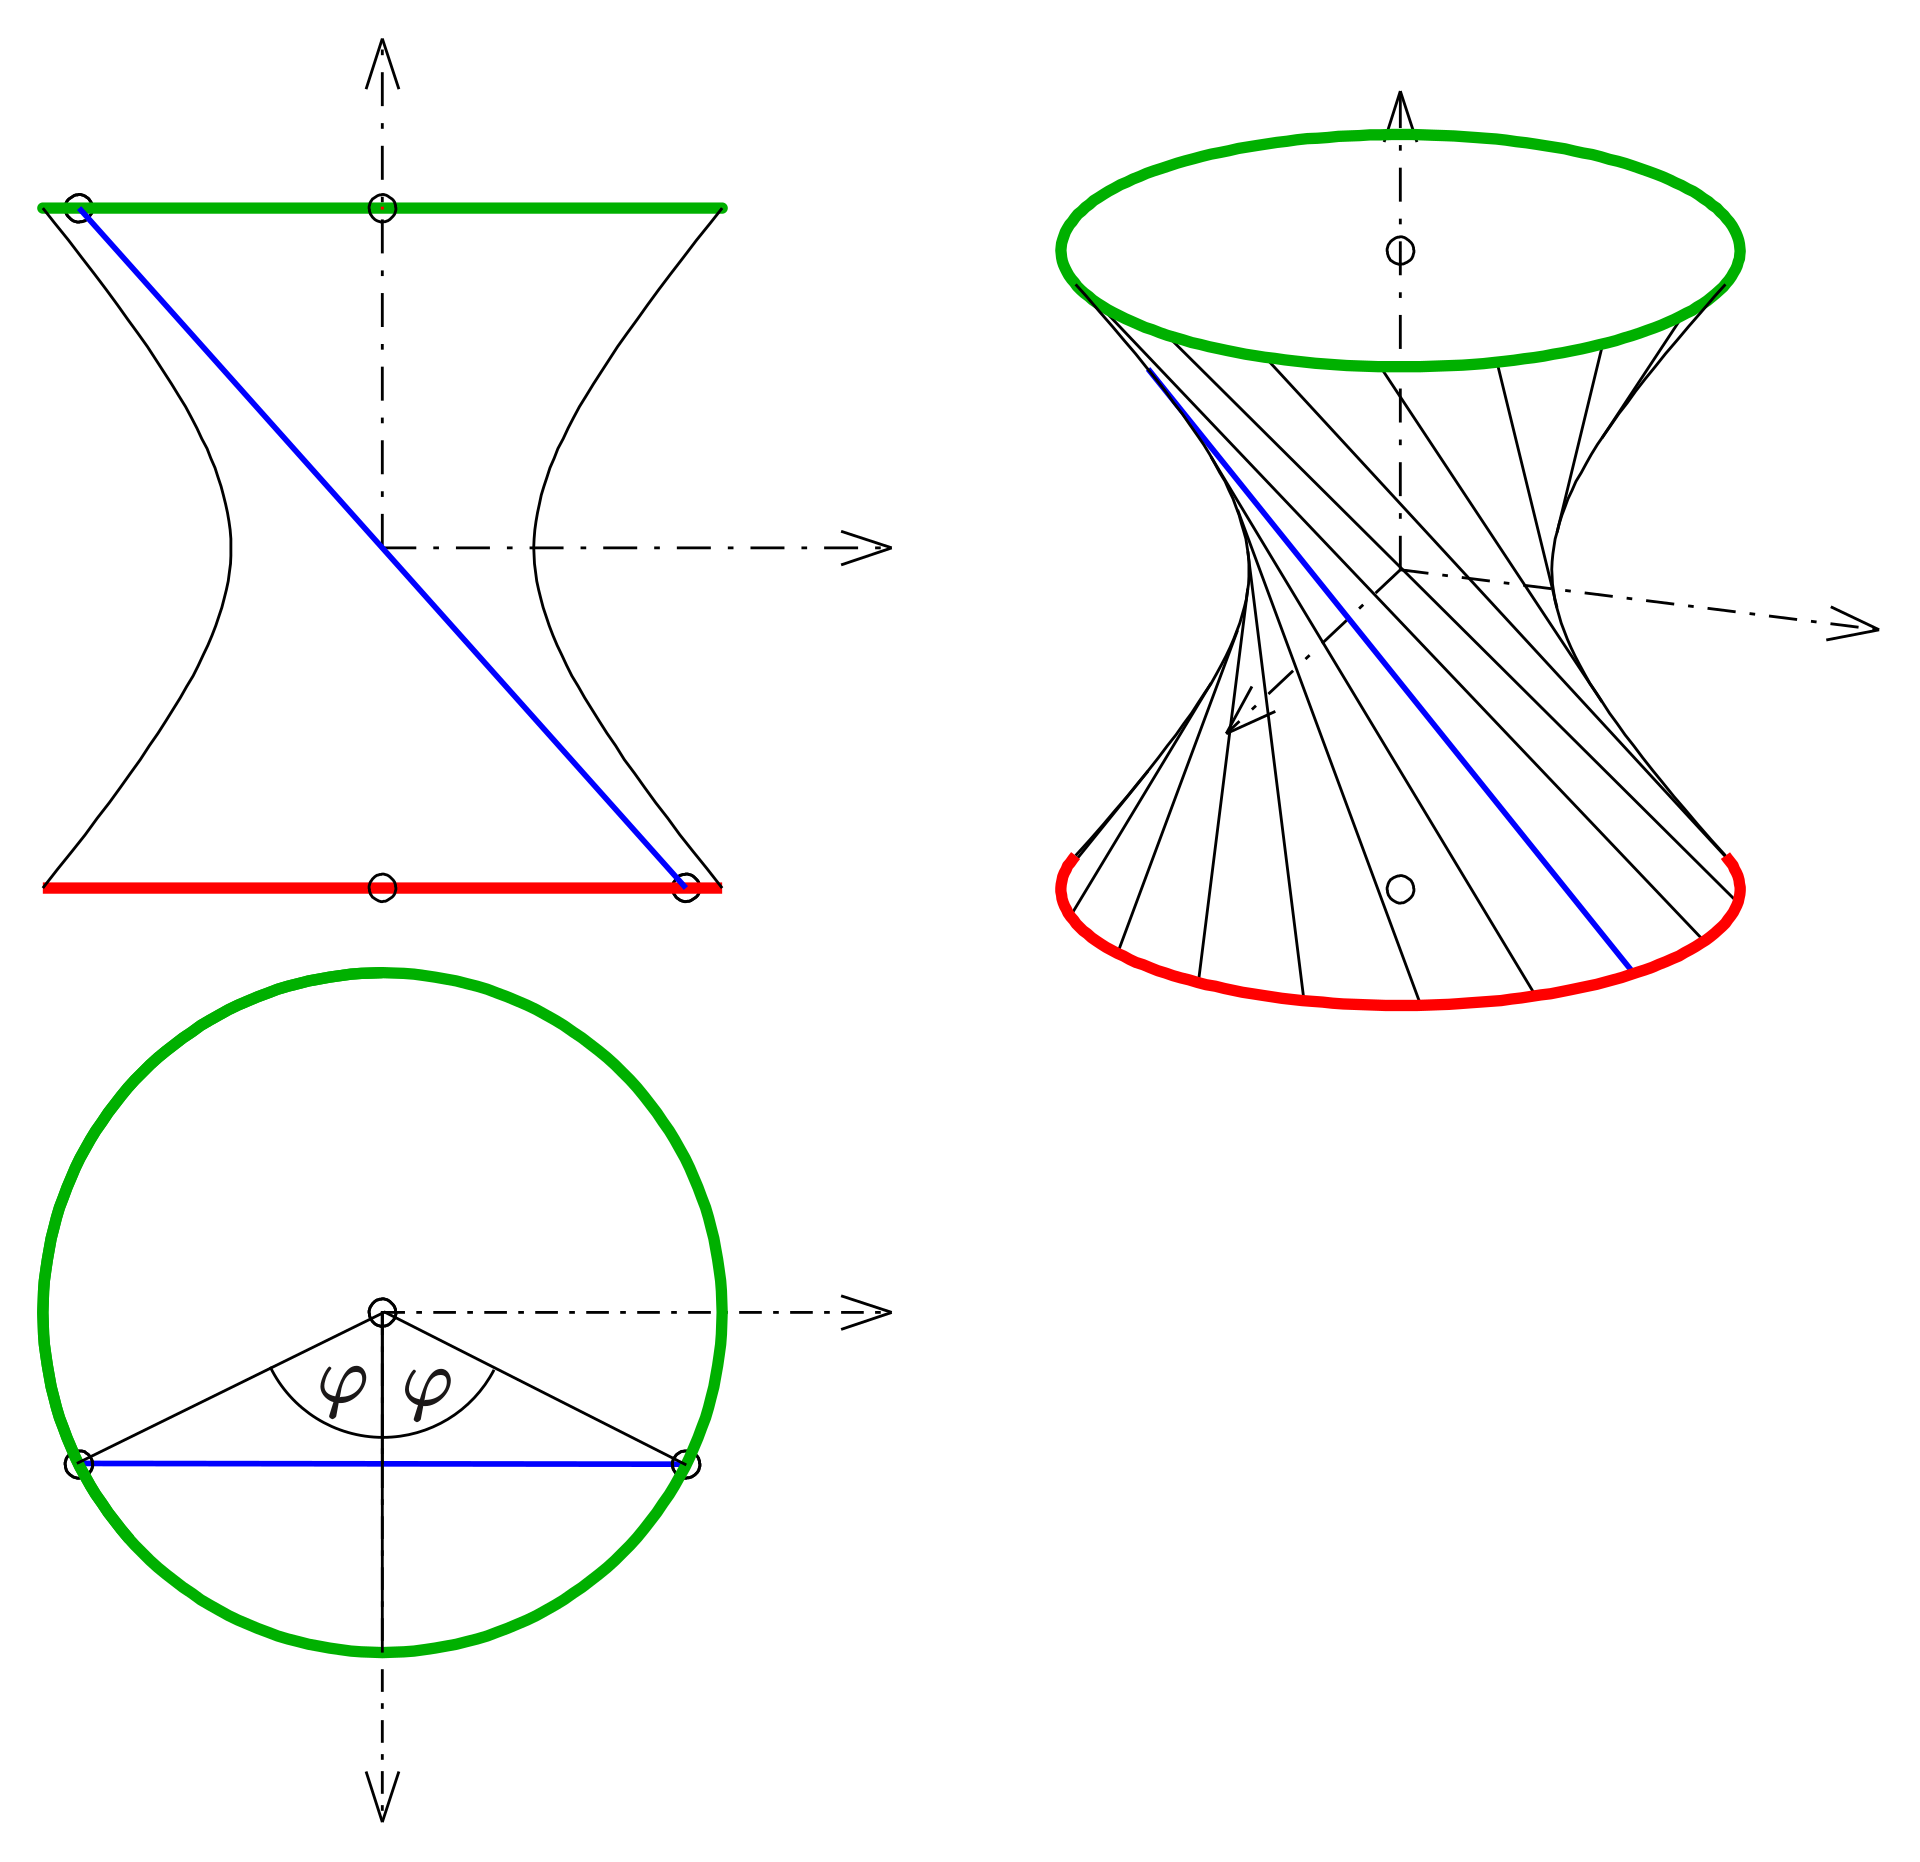
\includegraphics{./HyperboloidRuled.png}
\caption{HypRuled}
\end{figure}

Our steps are then:

\begin{itemize}
\tightlist
\item
  generate \(n\) points along 2 circumferences, with some phase
  difference between the corresponding points
\item
  draw a straight line connecting the couples of points of the
  circumference
\end{itemize}

    \begin{tcolorbox}[breakable, size=fbox, boxrule=1pt, pad at break*=1mm,colback=cellbackground, colframe=cellborder]
\prompt{In}{incolor}{ }{\boxspacing}
\begin{Verbatim}[commandchars=\\\{\}]
\PY{n+nb}{print}\PY{p}{(}\PY{l+s+s2}{\PYZdq{}}\PY{l+s+s2}{We define here a function which draws a circumference on the xy plane at height z}\PY{l+s+s2}{\PYZdq{}}\PY{p}{)}
\PY{k+kn}{import} \PY{n+nn}{numpy} \PY{k}{as} \PY{n+nn}{np}
\PY{k}{def} \PY{n+nf}{circ\PYZus{}points}\PY{p}{(}\PY{n}{n}\PY{p}{,} \PY{n}{phi}\PY{p}{,} \PY{n}{h}\PY{p}{)}\PY{p}{:}
  \PY{n}{points} \PY{o}{=} \PY{p}{[}\PY{p}{]} \PY{c+c1}{\PYZsh{} list of points}
  \PY{k}{for} \PY{n}{i} \PY{o+ow}{in} \PY{n+nb}{range}\PY{p}{(}\PY{l+m+mi}{0}\PY{p}{,}\PY{n}{n}\PY{p}{)}\PY{p}{:}
    \PY{n}{theta} \PY{o}{=} \PY{n}{phi} \PY{o}{+} \PY{n}{i}\PY{o}{*}\PY{p}{(}\PY{l+m+mi}{2}\PY{o}{*}\PY{n}{np}\PY{o}{.}\PY{n}{pi}\PY{o}{/}\PY{n}{n}\PY{p}{)} 
    \PY{n}{x} \PY{o}{=} \PY{n}{cos}\PY{p}{(}\PY{n}{theta}\PY{p}{)}
    \PY{n}{y} \PY{o}{=} \PY{n}{sin}\PY{p}{(}\PY{n}{theta}\PY{p}{)}
    \PY{n}{z} \PY{o}{=} \PY{n}{h}
    \PY{n}{points}\PY{o}{.}\PY{n}{append}\PY{p}{(}\PY{p}{[}\PY{n}{x}\PY{p}{,}\PY{n}{y}\PY{p}{,}\PY{n}{z}\PY{p}{]}\PY{p}{)}
  \PY{k}{return} \PY{n}{points}
   
\PY{n+nb}{print}\PY{p}{(}\PY{l+s+s2}{\PYZdq{}}\PY{l+s+s2}{Check of the function:}\PY{l+s+s2}{\PYZdq{}}\PY{p}{)}
\PY{n}{Pi} \PY{o}{=} \PY{n}{circ\PYZus{}points}\PY{p}{(}\PY{l+m+mi}{10}\PY{p}{,} \PY{l+m+mf}{0.0}\PY{p}{,} \PY{l+m+mf}{0.0}\PY{p}{)}
\PY{n+nb}{print}\PY{p}{(}\PY{n}{Pi}\PY{p}{)}
\end{Verbatim}
\end{tcolorbox}

    \begin{tcolorbox}[breakable, size=fbox, boxrule=1pt, pad at break*=1mm,colback=cellbackground, colframe=cellborder]
\prompt{In}{incolor}{ }{\boxspacing}
\begin{Verbatim}[commandchars=\\\{\}]
\PY{n+nb}{print}\PY{p}{(}\PY{l+s+s2}{\PYZdq{}}\PY{l+s+s2}{Here we define a function that plot a line passing for A and B}\PY{l+s+s2}{\PYZdq{}}\PY{p}{)}
\PY{k+kn}{import} \PY{n+nn}{numpy} \PY{k}{as} \PY{n+nn}{np}
\PY{k}{def} \PY{n+nf}{get\PYZus{}plot\PYZus{}line}\PY{p}{(}\PY{n}{A0}\PY{p}{,}\PY{n}{B0}\PY{p}{,} \PY{n}{I}\PY{o}{=}\PY{p}{[}\PY{o}{\PYZhy{}}\PY{l+m+mi}{5}\PY{p}{,}\PY{l+m+mi}{5}\PY{p}{]}\PY{p}{)}\PY{p}{:}
  \PY{n}{A} \PY{o}{=} \PY{n}{np}\PY{o}{.}\PY{n}{array}\PY{p}{(}\PY{n}{A0}\PY{p}{)}
  \PY{n}{B} \PY{o}{=} \PY{n}{np}\PY{o}{.}\PY{n}{array}\PY{p}{(}\PY{n}{B0}\PY{p}{)}
  \PY{n}{v} \PY{o}{=} \PY{p}{(}\PY{n}{A} \PY{o}{\PYZhy{}} \PY{n}{B}\PY{p}{)}
  \PY{n}{t} \PY{o}{=} \PY{n}{symbols}\PY{p}{(}\PY{l+s+s2}{\PYZdq{}}\PY{l+s+s2}{t}\PY{l+s+s2}{\PYZdq{}}\PY{p}{)}
  \PY{n}{rt} \PY{o}{=} \PY{n}{A} \PY{o}{+} \PY{n}{v}\PY{o}{*}\PY{n}{t}
  \PY{k}{return} \PY{n}{plot3d\PYZus{}parametric\PYZus{}line}\PY{p}{(}\PY{n}{rt}\PY{p}{[}\PY{l+m+mi}{0}\PY{p}{]}\PY{p}{,} \PY{n}{rt}\PY{p}{[}\PY{l+m+mi}{1}\PY{p}{]}\PY{p}{,} \PY{n}{rt}\PY{p}{[}\PY{l+m+mi}{2}\PY{p}{]}\PY{p}{,} \PY{p}{(}\PY{n}{t}\PY{p}{,} \PY{n}{I}\PY{p}{[}\PY{l+m+mi}{0}\PY{p}{]}\PY{p}{,} \PY{n}{I}\PY{p}{[}\PY{l+m+mi}{1}\PY{p}{]}\PY{p}{)}\PY{p}{,} \PY{n}{show}\PY{o}{=}\PY{k+kc}{False}\PY{p}{)}
  
  
\PY{n+nb}{print}\PY{p}{(}\PY{l+s+s2}{\PYZdq{}}\PY{l+s+s2}{testing}\PY{l+s+s2}{\PYZdq{}}\PY{p}{)}
\PY{n}{p1} \PY{o}{=} \PY{n}{get\PYZus{}plot\PYZus{}line}\PY{p}{(}\PY{p}{[}\PY{l+m+mi}{0}\PY{p}{,}\PY{l+m+mi}{0}\PY{p}{,}\PY{l+m+mi}{0}\PY{p}{]}\PY{p}{,}\PY{p}{[}\PY{l+m+mi}{1}\PY{p}{,}\PY{l+m+mi}{2}\PY{p}{,}\PY{l+m+mi}{3}\PY{p}{]}\PY{p}{)}
\PY{c+c1}{\PYZsh{} p1.show()}
\end{Verbatim}
\end{tcolorbox}

    \begin{tcolorbox}[breakable, size=fbox, boxrule=1pt, pad at break*=1mm,colback=cellbackground, colframe=cellborder]
\prompt{In}{incolor}{ }{\boxspacing}
\begin{Verbatim}[commandchars=\\\{\}]
\PY{n}{N} \PY{o}{=} \PY{l+m+mi}{40}
\PY{n}{phi} \PY{o}{=} \PY{l+m+mf}{0.5}
\PY{n}{h} \PY{o}{=} \PY{l+m+mi}{1}
\PY{n}{c1} \PY{o}{=} \PY{n}{circ\PYZus{}points}\PY{p}{(}\PY{n}{N}\PY{p}{,}\PY{l+m+mf}{0.0}\PY{p}{,}\PY{l+m+mf}{0.0}\PY{p}{)}
\PY{n}{c2} \PY{o}{=} \PY{n}{circ\PYZus{}points}\PY{p}{(}\PY{n}{N}\PY{p}{,}\PY{n}{phi}\PY{p}{,}\PY{n}{h}\PY{p}{)}

\PY{n}{P\PYZus{}hyp} \PY{o}{=} \PY{n}{sympy}\PY{o}{.}\PY{n}{plotting}\PY{o}{.}\PY{n}{plot}\PY{p}{(}\PY{n}{show}\PY{o}{=}\PY{k+kc}{False}\PY{p}{)}
\PY{k}{for} \PY{n}{i} \PY{o+ow}{in} \PY{n+nb}{range}\PY{p}{(}\PY{l+m+mi}{0}\PY{p}{,}\PY{n}{N}\PY{p}{)}\PY{p}{:}
    \PY{n}{P\PYZus{}hyp}\PY{o}{.}\PY{n}{extend}\PY{p}{(}\PY{n}{get\PYZus{}plot\PYZus{}line}\PY{p}{(}\PY{n}{c1}\PY{p}{[}\PY{n}{i}\PY{p}{]}\PY{p}{,} \PY{n}{c2}\PY{p}{[}\PY{n}{i}\PY{p}{]}\PY{p}{)}\PY{p}{)}
\PY{n}{P\PYZus{}hyp}\PY{o}{.}\PY{n}{show}\PY{p}{(}\PY{p}{)}
\end{Verbatim}
\end{tcolorbox}

    Now we can think to automate the process:

    \begin{tcolorbox}[breakable, size=fbox, boxrule=1pt, pad at break*=1mm,colback=cellbackground, colframe=cellborder]
\prompt{In}{incolor}{1}{\boxspacing}
\begin{Verbatim}[commandchars=\\\{\}]
\PY{n+nb}{print}\PY{p}{(}\PY{l+s+s2}{\PYZdq{}}\PY{l+s+s2}{Defining a function for generic hyperboloid as ruled surface}\PY{l+s+s2}{\PYZdq{}}\PY{p}{)}
\PY{k}{def} \PY{n+nf}{hyp\PYZus{}ruled}\PY{p}{(}\PY{n}{N}\PY{p}{,} \PY{n}{phi}\PY{p}{,} \PY{n}{h}\PY{p}{)}\PY{p}{:}
    \PY{n}{c1} \PY{o}{=} \PY{n}{circ\PYZus{}points}\PY{p}{(}\PY{n}{N}\PY{p}{,}\PY{l+m+mf}{0.0}\PY{p}{,}\PY{l+m+mf}{0.0}\PY{p}{)}
    \PY{n}{c2} \PY{o}{=} \PY{n}{circ\PYZus{}points}\PY{p}{(}\PY{n}{N}\PY{p}{,}\PY{n}{phi}\PY{p}{,}\PY{n}{h}\PY{p}{)}
    \PY{n}{P\PYZus{}hyp} \PY{o}{=} \PY{n}{sympy}\PY{o}{.}\PY{n}{plotting}\PY{o}{.}\PY{n}{plot}\PY{p}{(}\PY{n}{show}\PY{o}{=}\PY{k+kc}{False}\PY{p}{)}
    \PY{k}{for} \PY{n}{i} \PY{o+ow}{in} \PY{n+nb}{range}\PY{p}{(}\PY{l+m+mi}{0}\PY{p}{,}\PY{n}{N}\PY{p}{)}\PY{p}{:}
        \PY{n}{P\PYZus{}hyp}\PY{o}{.}\PY{n}{extend}\PY{p}{(}\PY{n}{get\PYZus{}plot\PYZus{}line}\PY{p}{(}\PY{n}{c1}\PY{p}{[}\PY{n}{i}\PY{p}{]}\PY{p}{,} \PY{n}{c2}\PY{p}{[}\PY{n}{i}\PY{p}{]}\PY{p}{)}\PY{p}{)}
    \PY{n}{P\PYZus{}hyp}\PY{o}{.}\PY{n}{show}\PY{p}{(}\PY{p}{)}
    
\end{Verbatim}
\end{tcolorbox}

    \begin{Verbatim}[commandchars=\\\{\}]
Defining a function for generic hyperboloid as ruled surface
    \end{Verbatim}

    \begin{tcolorbox}[breakable, size=fbox, boxrule=1pt, pad at break*=1mm,colback=cellbackground, colframe=cellborder]
\prompt{In}{incolor}{2}{\boxspacing}
\begin{Verbatim}[commandchars=\\\{\}]
\PY{n+nb}{print}\PY{p}{(}\PY{l+s+s2}{\PYZdq{}}\PY{l+s+s2}{Testing:}\PY{l+s+s2}{\PYZdq{}}\PY{p}{)}

\PY{n}{hyp\PYZus{}ruled}\PY{p}{(}\PY{l+m+mi}{40}\PY{p}{,} \PY{l+m+mf}{1.0}\PY{p}{,} \PY{l+m+mi}{25}\PY{p}{)}
\end{Verbatim}
\end{tcolorbox}

    \begin{Verbatim}[commandchars=\\\{\}]
Testing:
    \end{Verbatim}

    \begin{Verbatim}[commandchars=\\\{\}]

        ---------------------------------------------------------------------------

        NameError                                 Traceback (most recent call last)

        <ipython-input-2-25b3985cfade> in <module>
          1 print("Testing:")
          2 
    ----> 3 hyp\_ruled(40, 1.0, 25)
    

        <ipython-input-1-17a9137e00f8> in hyp\_ruled(N, phi, h)
          1 print("Defining a function for generic hyperboloid as ruled surface")
          2 def hyp\_ruled(N, phi, h):
    ----> 3     c1 = circ\_points(N,0.0,0.0)
          4     c2 = circ\_points(N,phi,h)
          5     P\_hyp = sympy.plotting.plot(show=False)


        NameError: name 'circ\_points' is not defined

    \end{Verbatim}

    \begin{tcolorbox}[breakable, size=fbox, boxrule=1pt, pad at break*=1mm,colback=cellbackground, colframe=cellborder]
\prompt{In}{incolor}{ }{\boxspacing}
\begin{Verbatim}[commandchars=\\\{\}]

\end{Verbatim}
\end{tcolorbox}

    \begin{tcolorbox}[breakable, size=fbox, boxrule=1pt, pad at break*=1mm,colback=cellbackground, colframe=cellborder]
\prompt{In}{incolor}{ }{\boxspacing}
\begin{Verbatim}[commandchars=\\\{\}]

\end{Verbatim}
\end{tcolorbox}

    \begin{tcolorbox}[breakable, size=fbox, boxrule=1pt, pad at break*=1mm,colback=cellbackground, colframe=cellborder]
\prompt{In}{incolor}{ }{\boxspacing}
\begin{Verbatim}[commandchars=\\\{\}]

\end{Verbatim}
\end{tcolorbox}

    \begin{tcolorbox}[breakable, size=fbox, boxrule=1pt, pad at break*=1mm,colback=cellbackground, colframe=cellborder]
\prompt{In}{incolor}{ }{\boxspacing}
\begin{Verbatim}[commandchars=\\\{\}]

\end{Verbatim}
\end{tcolorbox}

    \begin{tcolorbox}[breakable, size=fbox, boxrule=1pt, pad at break*=1mm,colback=cellbackground, colframe=cellborder]
\prompt{In}{incolor}{ }{\boxspacing}
\begin{Verbatim}[commandchars=\\\{\}]

\end{Verbatim}
\end{tcolorbox}


    % Add a bibliography block to the postdoc
    
    
    
\end{document}
